% !TeX root = ..\main.tex
\section{Thiết kế giao diện}

\subsection{Giao diện chung}
\subsubsection{Đăng nhập}
\begin{figure}[!htp]
    \centering
    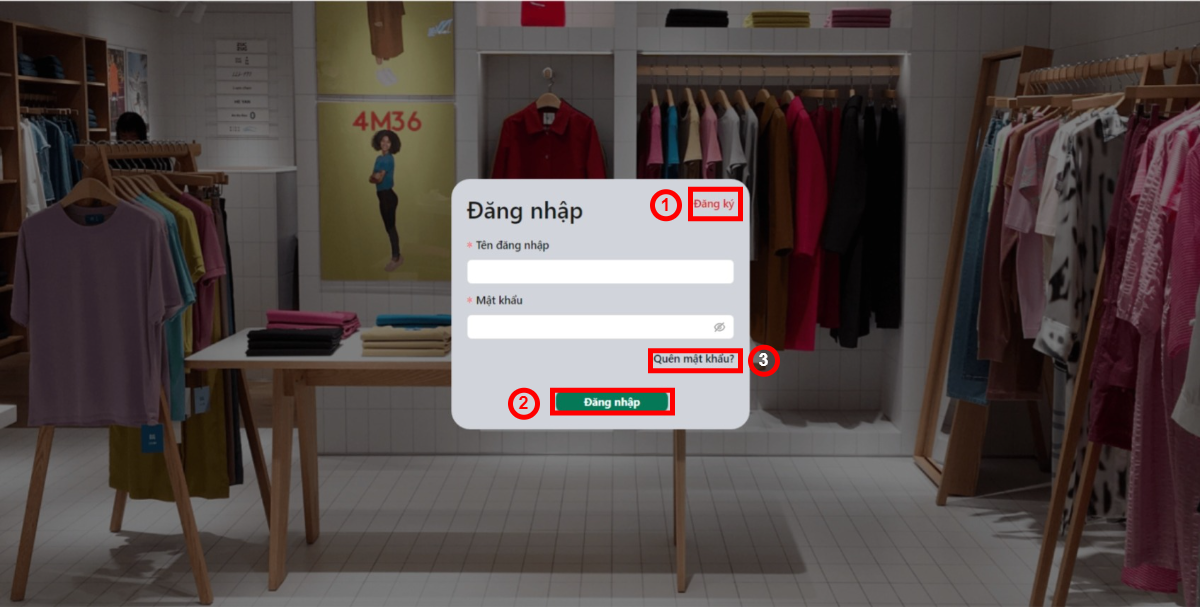
\includegraphics[width=5in]{img/UI/new_customer/login.png}
    \label{1}
    \newline
    \caption{Giao diện đăng nhập}
\end{figure}
\textbf{Mô tả:}
\begin{quote}
    \begin{enumerate}
        \item Chọn để chuyển tới trang đăng ký tài khoản.
              % \item Nhập tên đăng nhập của tài khoản, yêu cầu tối thiểu 1 ký tự.
              % \item Nhập mật khẩu của tài khoản, yêu cầu mật khẩu tối thiểu 6 ký tự.
        \item Chọn để thực hiện đăng nhập tài khoản, nếu thông tin tài khoản đúng thì sẽ được đưa đến giao diện mặc định cho tài khoản.
        \item Chọn "Quên mật khẩu" khi không nhớ mật khẩu của tài khoản để chuyển trang sang trang lấy lại mật khẩu.
    \end{enumerate}
\end{quote}




\subsection{Giao diện người dùng}
\subsubsection{Đăng ký}
\begin{figure}[!htp]
    \centering
    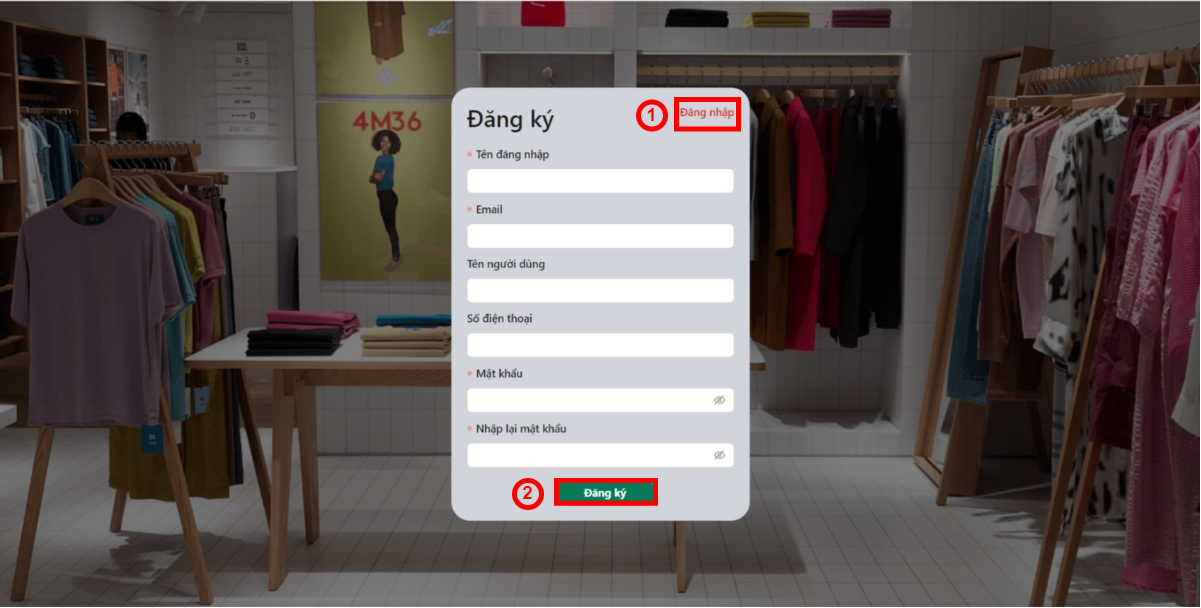
\includegraphics[width=5in]{img/UI/new_customer/register.png}
    \label{2}
    \newline
    \caption{Giao diện đăng ký tài khoản người dùng}
\end{figure}
\textbf{Mô tả:}
\begin{quote}
    \begin{enumerate}
        \item Chọn để chuyển tới trang đăng đăng nhập.
              % \item Nhập tên đăng nhập của tài khoản, yêu cầu tối thiểu một ký tự.
              % \item Nhập tên của người dùng, yêu cầu tối thiểu một ký tự.
              % \item Nhập số điện thoại của người dùng, yêu cầu đúng định dạng số điện thoại 10 chữ số, bắt đầu bằng số 09 / 03 / 05 / 07 / 08.
              % \item Nhập mật khẩu của tài khoản, yêu cầu tối thiểu 6 ký tự.
              % \item Nhập lại mật khẩu của tài khoản, yêu cầu phải giống mật khẩu của tài khoản đã nhập.
        \item Chọn để thực hiện đăng ký tài khoản, nếu đăng ký thành công thì chuyển tới trang đăng nhập.
    \end{enumerate}
\end{quote}


\subsubsection{Tạo lại mật khẩu}
\begin{figure}[!htp]
    \centering
    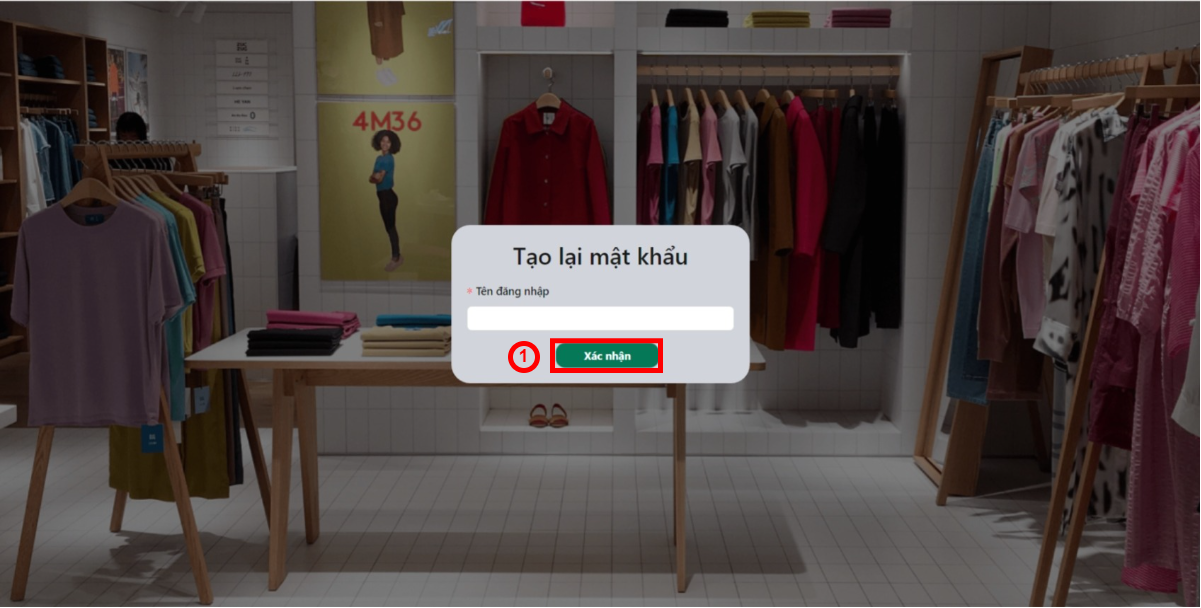
\includegraphics[width=5in]{img/UI/new_customer/reset_password.png}
    \label{3}
    \newline
    \caption{Giao diện tạo lại mật khẩu người dùng}
\end{figure}
\textbf{Mô tả:}
\begin{quote}
    \begin{enumerate}
        \item Người dùng nhập số điện thoại của tài khoản, yêu cầu đúng định dạng số điện thoại 10 chữ số, bắt đầu bằng số 09 / 03 / 05 / 07 / 08.
        \item Người dùng chọn để hệ thống gửi xác nhận tin nhắn OTP và chuyển tới trang xác nhận OTP.
    \end{enumerate}
\end{quote}


\begin{figure}[!htp]
    \centering
    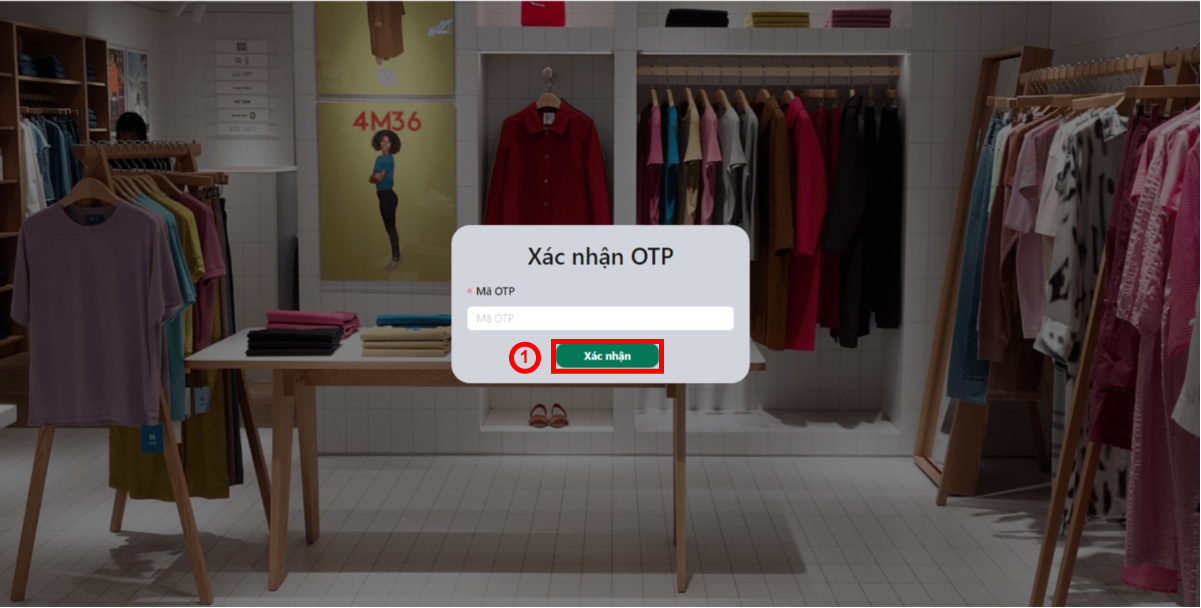
\includegraphics[width=5in]{img/UI/new_customer/confirm_otp.png}
    \label{4}
    \newline
    \caption{Giao diện xác nhận OTP}
\end{figure}
\textbf{Mô tả:}
\begin{quote}
    \begin{enumerate}
        \item Người dùng nhập OTP đã được gửi qua tin nhắn, yêu cầu 6 ký tự.
        \item Người dùng chọn để hệ thống xác nhận và thông tin hợp lệ sẽ được gửi mail với mật khẩu mới cho tài khoản và chuyển đến trang đăng nhập.
    \end{enumerate}
\end{quote}
% \textbf{Mô tả:}
% \begin{quote}
%     \begin{enumerate}
%         \item Người dùng nhập số điện thoại của tài khoản, yêu cầu đúng định dạng số điện thoại 10 chữ số, bắt đầu bằng số 09 / 03 / 05 / 07 / 08.
%         \item Người dùng chọn để hệ thống gửi xác nhận tin nhắn OTP và chuyển tới trang xác nhận OTP.
%     \end{enumerate}
% \end{quote}
% \begin{figure}[!htp]
%     \centering
%     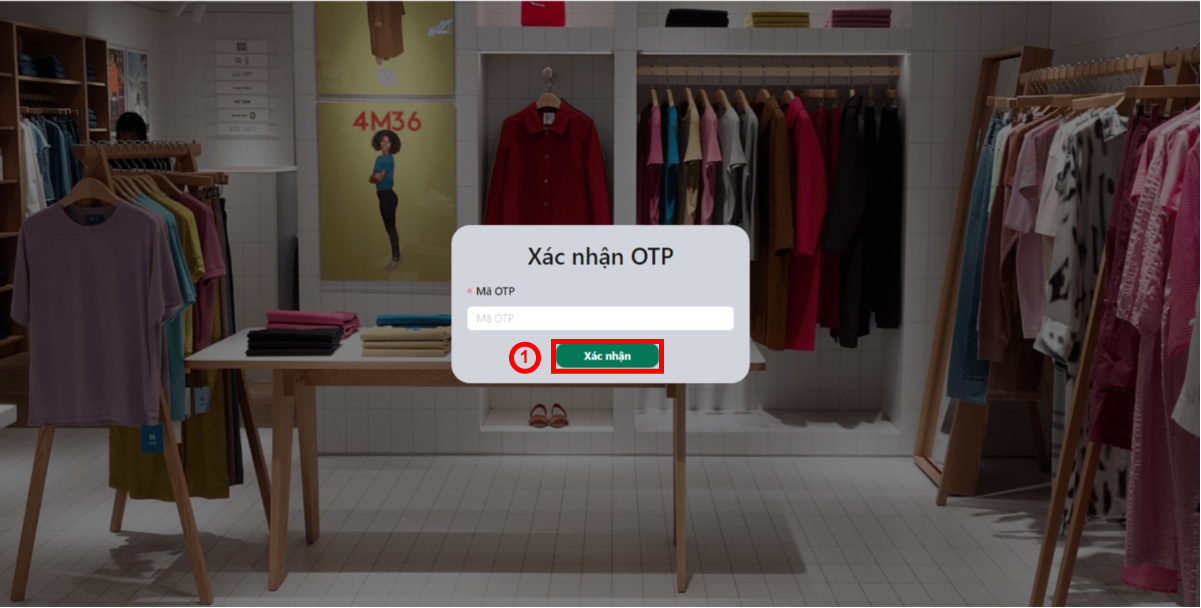
\includegraphics[width=5in]{img/UI/new_customer/confirm_otp.png}
%     \label{5}
%     \newline
%     \caption{Giao diện tạo lại mật khẩu mới}
% \end{figure}
% \textbf{Mô tả:}
% \begin{quote}
%     \begin{enumerate}
%         \item Người dùng nhập mật khẩu mới cho tài khoản, yêu cầu tối thiểu 6 ký tự.
%         \item Người dùng nhập lại mật khẩu mới cho tài khoản, yêu cầu phải giống với mật khẩu mới.
%         \item Người dùng chọn "Xác nhận" để cập nhật lại mật khẩu mới cho tài khoản.
%     \end{enumerate}
% \end{quote}

\subsubsection{Header}
\begin{figure}[!htp]
    \centering
    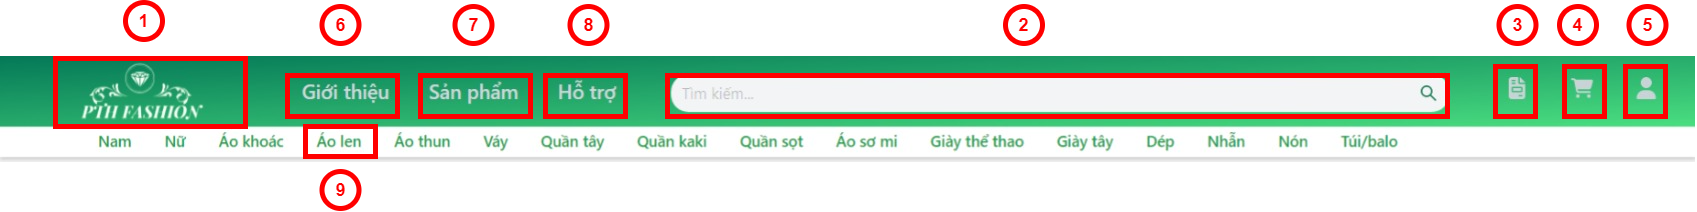
\includegraphics[width=5in]{img/UI/new_customer/header.png}
    \label{6}
    \newline
    \caption{Giao diện phần header}
\end{figure}
\textbf{Mô tả:}
\begin{quote}
    \begin{enumerate}
        \item Chọn để chuyển tới trang chủ.
        \item Nhập tên sản phẩm cần tìm và nhấn enter để tìm kiếm sản phẩm.
        \item Chọn để chuyển đến trang quản lý lịch sử đơn hàng đã thực hiện.
        \item Chọn để chuyển đến trang quản lý giỏ hàng.
        \item Chọn để đăng nhập / xem thông tin cá nhân tài khoản.
        \item Chọn để chuyển đến trang giới thiệu về hệ thống cửa hàng.
        \item Chọn để chuyển đến trang tất cả sản phẩm.
        \item Chọn để chuyển đến trang hỗ trợ.
        \item Chọn để chuyển đến trang tất cả sản phẩm với lựa chọn lọc sẵn là sản phẩm thuộc áo len.
    \end{enumerate}
\end{quote}

\subsubsection{Footer}
\begin{figure}[!htp]
    \centering
    
\includegraphics[width=5in]{img/UI/new_customer/footer.png}
    \label{7}
    \newline
    \caption{Giao diện phần footer}
\end{figure}
\textbf{Mô tả:}
\begin{quote}
    \begin{enumerate}
        \item Chọn để chuyển tới trang chủ.
        \item Chọn để chuyển đến trang tất cả sản phẩm.
        \item Chọn để chuyển đến trang hỗ trợ cho khách hàng.
        \item Chọn để chuyển đến trang giới thiệu về hệ thống cửa hàng.
        \item Chọn để xem hướng dẫn chọn size.
        \item Chọn để chuyển đến trang quản lý lịch sử đơn hàng đã thực hiện.
    \end{enumerate}
\end{quote}

\newpage
\subsubsection{Trang chủ}
\begin{figure}[!htp]
    \centering
    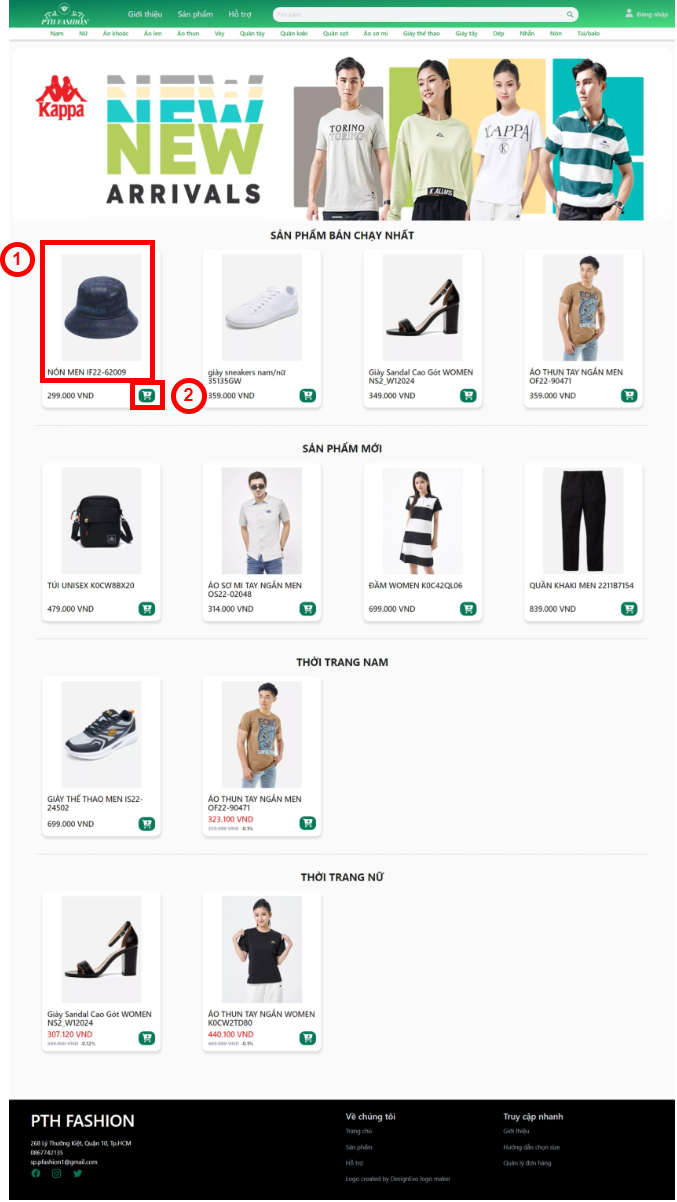
\includegraphics[width=3.5in]{img/UI/new_customer/home.png}
    \label{8}
    \newline
    \caption{Giao diện trang chủ khi người dùng truy cập vào trang web}
\end{figure}
\textbf{Mô tả:}
\begin{quote}
    \begin{enumerate}
        \item Chọn để xem thông tin chi tiết của sản phẩm.
        \item Chọn để thêm nhanh sản phẩm vào giỏ hàng.
    \end{enumerate}
\end{quote}

\subsubsection{Thông tin chi tiết sản phẩm}
\begin{figure}[!htp]
    \centering
    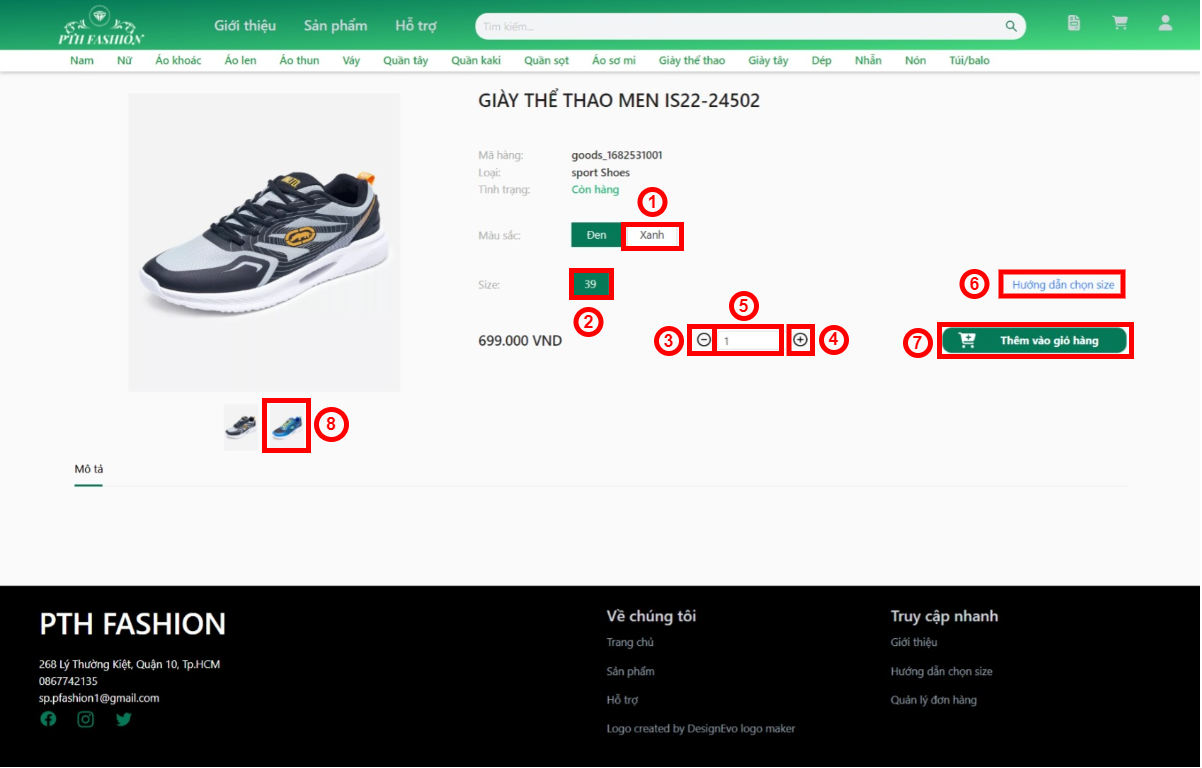
\includegraphics[width=5in]{img/UI/new_customer/product_detail.png}
    \label{9}
    \newline
    \caption{Giao diện thông tin chi tiết của sản phẩm}
\end{figure}
\textbf{Mô tả:}
\begin{quote}
    \begin{enumerate}
        \item Chọn màu của sản phẩm mà người dùng muốn.
        \item Chọn size của sản phẩm mà người dùng muốn.
        \item Chọn để giảm số lượng mà người dùng muốn.
        \item Chọn để tăng số lượng mà người dùng muốn.
        \item Nhập để thay đổi số lượng mà người dùng muốn.
        \item Chọn để xem hướng dẫn chọn size cho sản phẩm.
        \item Chọn để thêm sản phẩm với màu sắc, size và số lượng mà người dùng đã chọn.
        \item Chọn để xem ảnh chi tiết mà người dùng muốn.
    \end{enumerate}
\end{quote}

\begin{figure}[!htp]
    \centering
    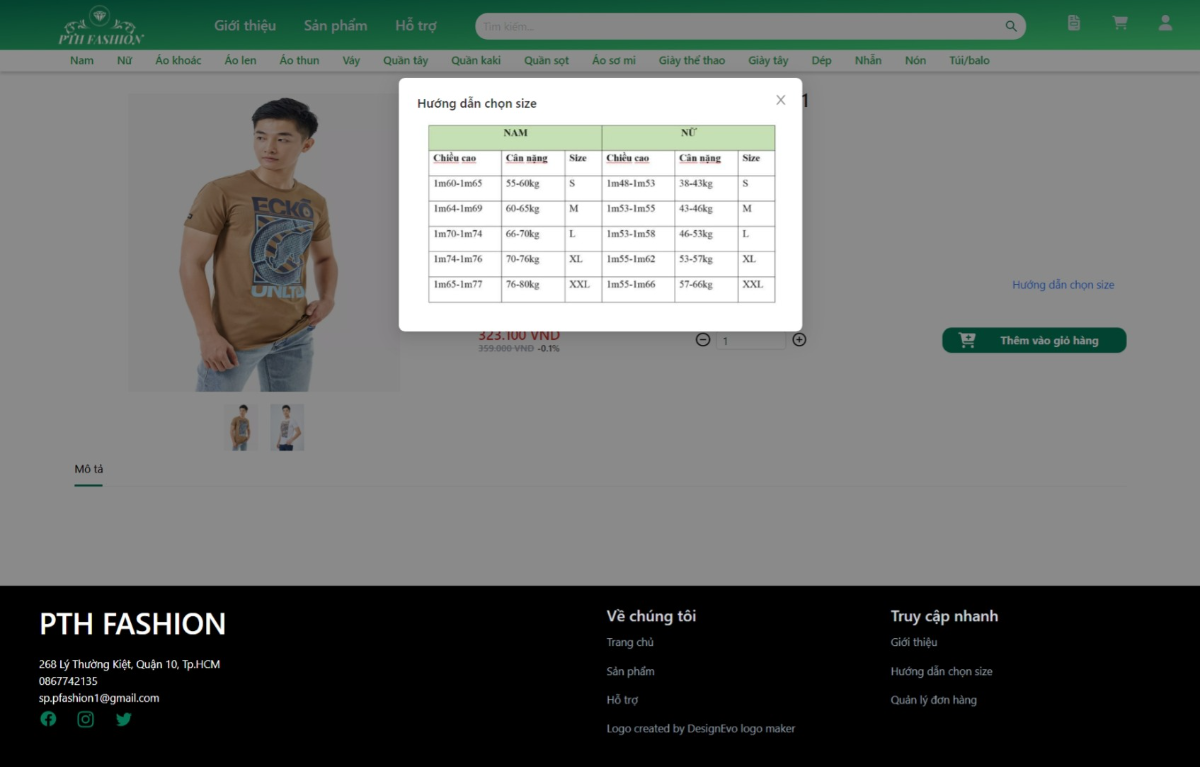
\includegraphics[width=5in]{img/UI/new_customer/guide_size.png}
    \label{10}
    \newline
    \caption{Giao diện hướng dẫn chọn size cho sản phẩm}
\end{figure}
\newpage

\subsubsection{Giỏ hàng}
\begin{figure}[!htp]
    \centering
    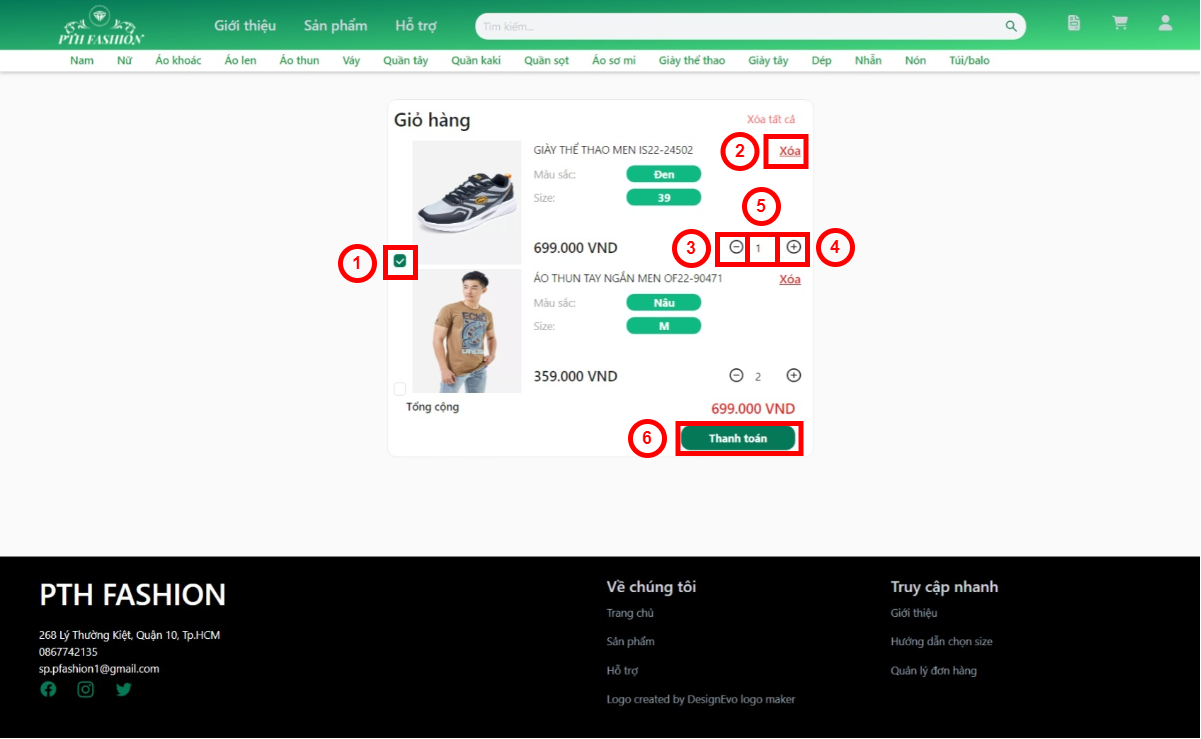
\includegraphics[width=5in]{img/UI/new_customer/cart.png}
    \label{11}
    \newline
    \caption{Giao diện quản lý giỏ hàng.}
\end{figure}
\textbf{Mô tả:}
\begin{quote}
    \begin{enumerate}
        \item Chọn để thêm/loại sản phẩm khỏi danh sách muốn đặt hàng.
        \item Chọn để xóa sản phẩm khỏi giỏ hàng.
        \item Chọn để giảm số lượng mà người dùng muốn.
        \item Chọn để tăng số lượng mà người dùng muốn.
        \item Nhập để thay đổi số lượng mà người dùng muốn.
              % \item Nhập mã giảm giá.
              % \item Chọn để áp dụng mã giảm giá.
        \item Chọn để thực hiện thanh toán để đặt hàng.
    \end{enumerate}
\end{quote}


\newpage

\subsubsection{Thanh toán}
\begin{figure}[!htp]
    \centering
    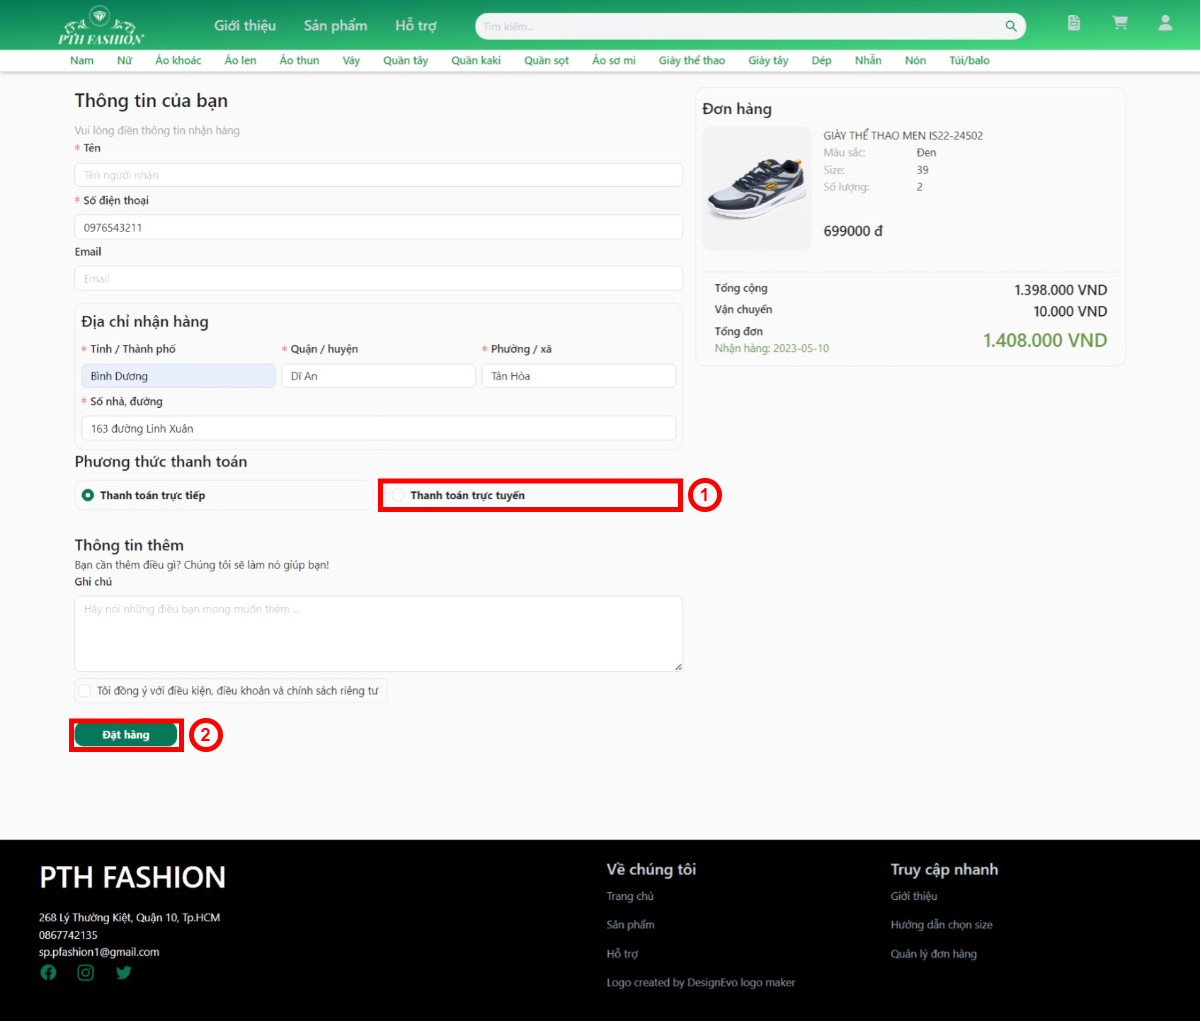
\includegraphics[width=5in]{img/UI/new_customer/payment.png}
    \label{12}
    \newline
    \caption{Giao diện thanh toán.}
\end{figure}
\textbf{Mô tả:}
\begin{quote}
    \begin{enumerate}
        % \item Nhập tên người nhận hàng.
        % \item Nhập số điện thoại người nhận hàng.
        % \item Nhập địa chỉ email người nhận hàng.
        % \item Nhập địa chỉ tỉnh/thành nhận hàng.
        % \item Nhập địa chỉ quận/huyện nhận hàng.
        % \item Nhập địa chỉ phường/xã nhận hàng.
        % \item Nhập địa chỉ số nhà, tên đường nhận hàng.
        \item Chọn để thực hiện thanh toán trực tuyến.
              % \item Chọn để thực hiện thanh toán trực tiếp khi nhận hàng.
              % \item Chọn để thực hiện thanh toán trực tuyến thông qua VNPay.
              % \item Chọn để thực hiện thanh toán trực tuyến thông qua Momo.
              % \item Nhập để thêm ghi chú cho đơn hàng.
              % \item Chọn để xác nhận đồng ý điều khoản mua hàng.
              % \item Nhập mã giảm giá.
              % \item Chọn để kiểm tra mã giảm giá và áp dụng giảm giá vào đơn hàng.
        \item Chọn để xác nhận đặt hàng, nếu chọn thanh toán trực tuyến thì sẽ được chuyển đến trang thanh toán của bên thứ ba mà người dùng chọn, nếu chọn thanh toán khi nhận hàng thì đơn hàng sẽ được hoàn tất khi tất cả thông tin hợp lệ.
    \end{enumerate}
\end{quote}


\newpage

\subsubsection{Giao diện quản lý đơn hàng}
\begin{figure}[!htp]
    \centering
    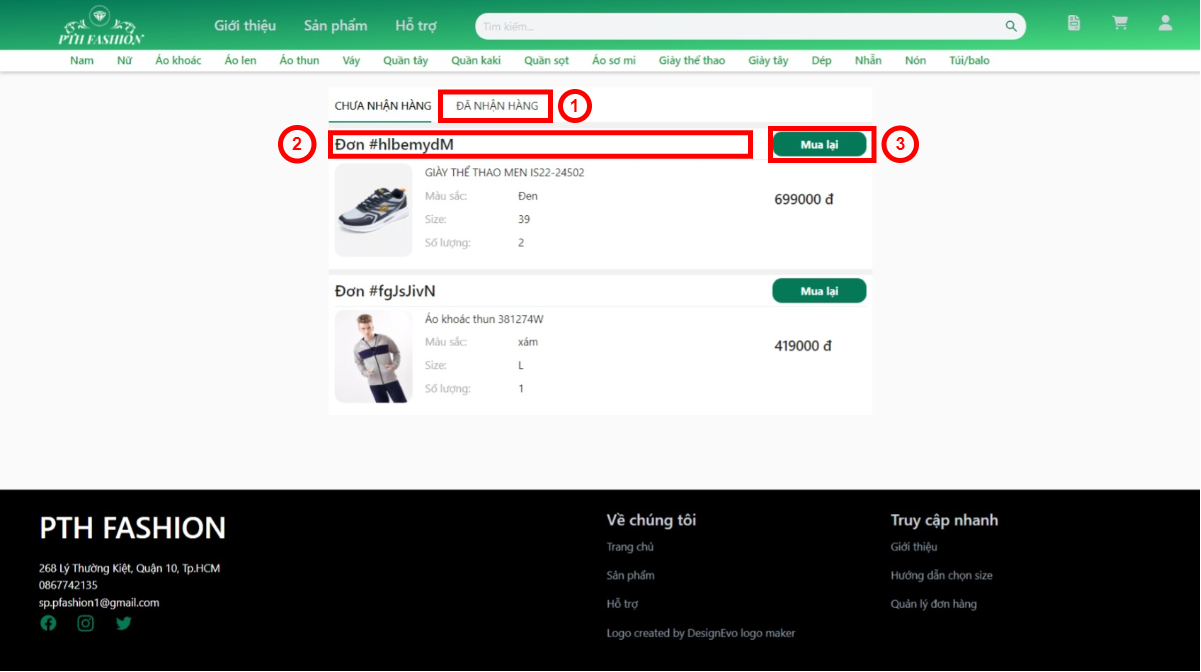
\includegraphics[width=5in]{img/UI/new_customer/customer_order.png}
    \label{13}
    \newline
    \caption{Giao diện quản lý đơn hàng của khách hàng.}
\end{figure}
\textbf{Mô tả:}
\begin{quote}
    \begin{enumerate}
        \item Chọn để xem danh sách các đơn hàng đã nhận.
        \item Chọn để xem thông tin chi tiết của đơn hàng.
        \item Chọn để thực hiện thêm lại các sản phẩm của đơn hàng vào giỏ hàng và chuyển đến trang giỏ hàng.
    \end{enumerate}
\end{quote}


\subsubsection{Giao diện chi tiết đơn hàng}
\begin{figure}[!htp]
    \centering
    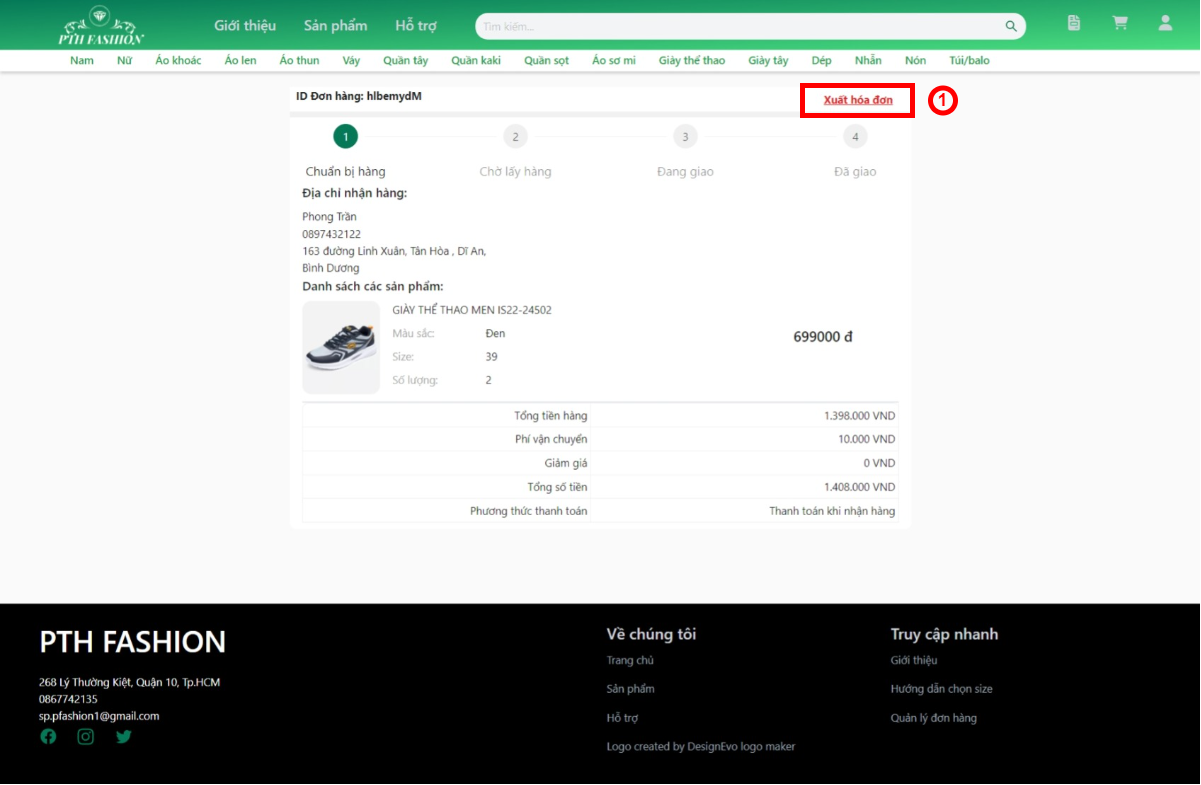
\includegraphics[width=5in]{img/UI/new_customer/order_detail.png}
    \label{14}
    \newline
    \caption{Giao diện xem chi tiết đơn hàng của khách hàng.}
\end{figure}
\textbf{Mô tả:}
\begin{quote}
    \begin{enumerate}
        \item Chọn để xuất hóa đơn cho đơn hàng.
    \end{enumerate}
\end{quote}
\newpage

\begin{figure}[!htp]
    \centering
    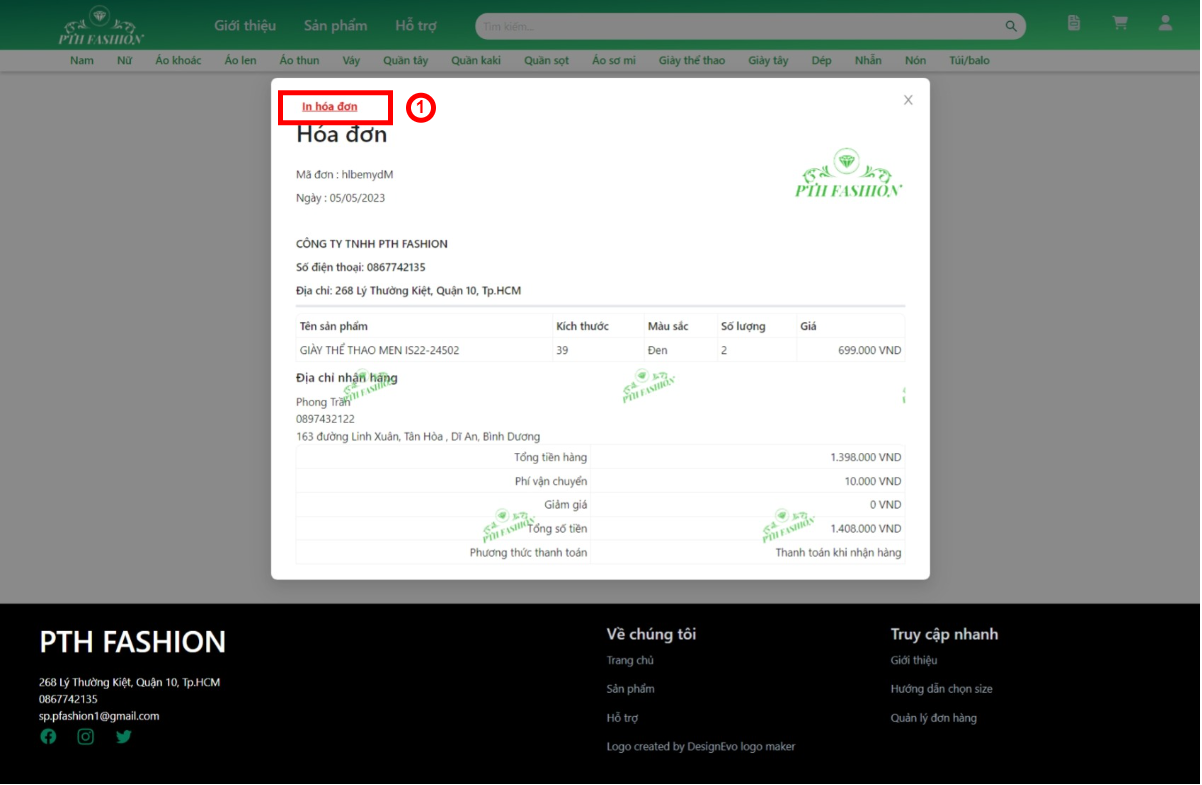
\includegraphics[width=5in]{img/UI/new_customer/invoice.png}
    \label{14}
    \newline
    \caption{Giao diện xuất hóa đơn.}
\end{figure}
\textbf{Mô tả:}
\begin{quote}
    \begin{enumerate}
        \item Chọn để in hóa đơn cho đơn hàng.
    \end{enumerate}
\end{quote}
\begin{figure}[!htp]
    \centering
    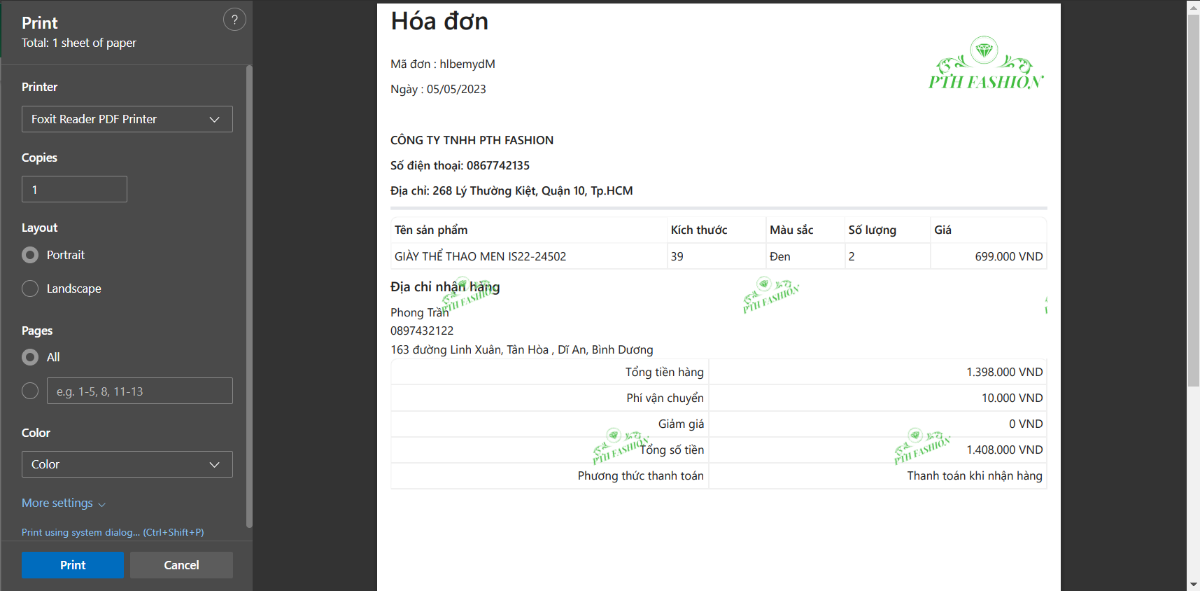
\includegraphics[width=5in]{img/UI/new_customer/print_invoice.png}
    \label{14}
    \newline
    \caption{Giao diện in hóa đơn khi chọn in hóa đơn.}
\end{figure}

\newpage

\subsubsection{Giao diện thông tin khách hàng}
\begin{figure}[!htp]
    \centering
    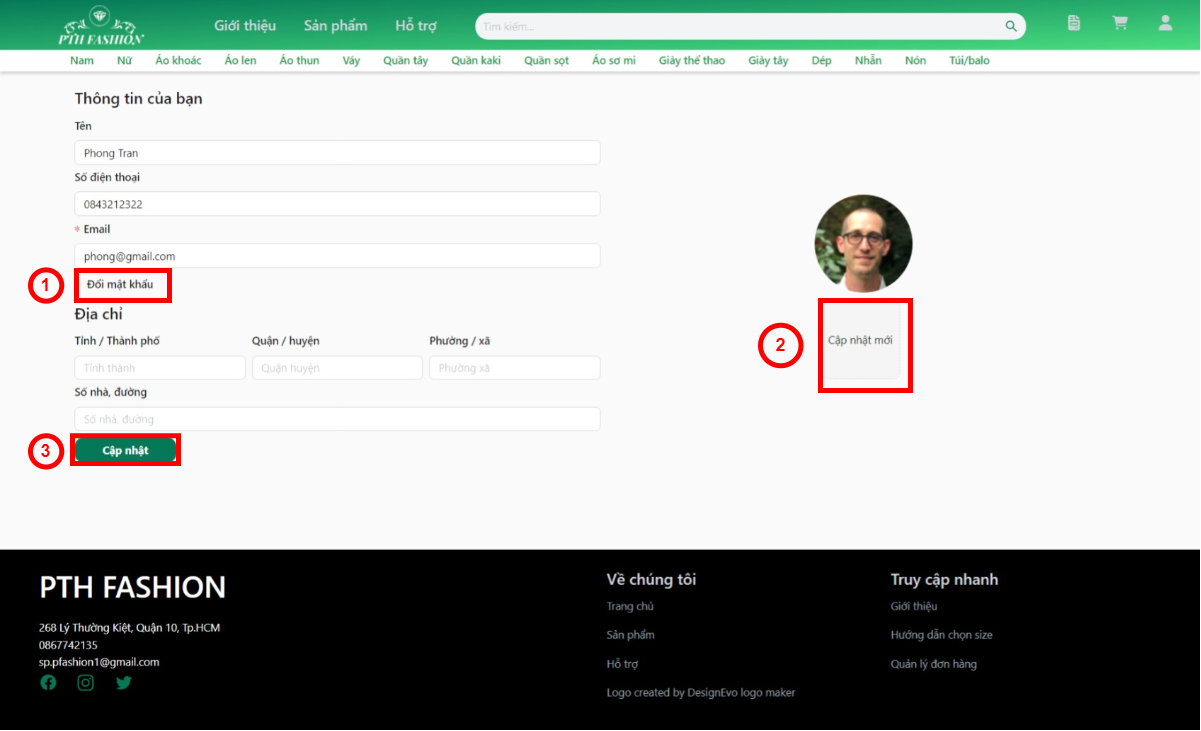
\includegraphics[width=5in]{img/UI/new_customer/customer_info.png}
    \label{15}
    \newline
    \caption{Giao diện xem thông tin tài khoản của khách hàng.}
\end{figure}
\textbf{Mô tả:}
\begin{quote}
    \begin{enumerate}
        % \item Nhập để thay đổi tên của khách hàng.
        % \item Nhập để thay đổi email của khách hàng.
        \item Chọn để thực hiện thay đổi mật khẩu của khách hàng.
              % \item Nhập để thay đổi số nhà, đường của địa chỉ mặc định mà khách hàng muốn nhận hàng.
              % \item Chọn để thay đổi phường/xã của địa chỉ mặc định mà khách hàng muốn nhận hàng.
              % \item Chọn để thay đổi quận/huyện của địa chỉ mặc định mà khách hàng muốn nhận hàng.
              % \item Chọn để thay đổi tỉnh/thành phố của địa chỉ mặc định mà khách hàng muốn nhận hàng.
        \item Chọn để thay đổi ảnh đại hình cho tài khoản của khách hàng.
        \item Chọn để xác nhận cập nhật thông tin đã chỉnh sửa.
    \end{enumerate}
\end{quote}

\newpage
\subsection{Giao diện quản trị viên}
\subsubsection{Chung}
\subsubsubsection{Thay đổi mật khẩu}
\begin{figure}[!htp]
    \centering
    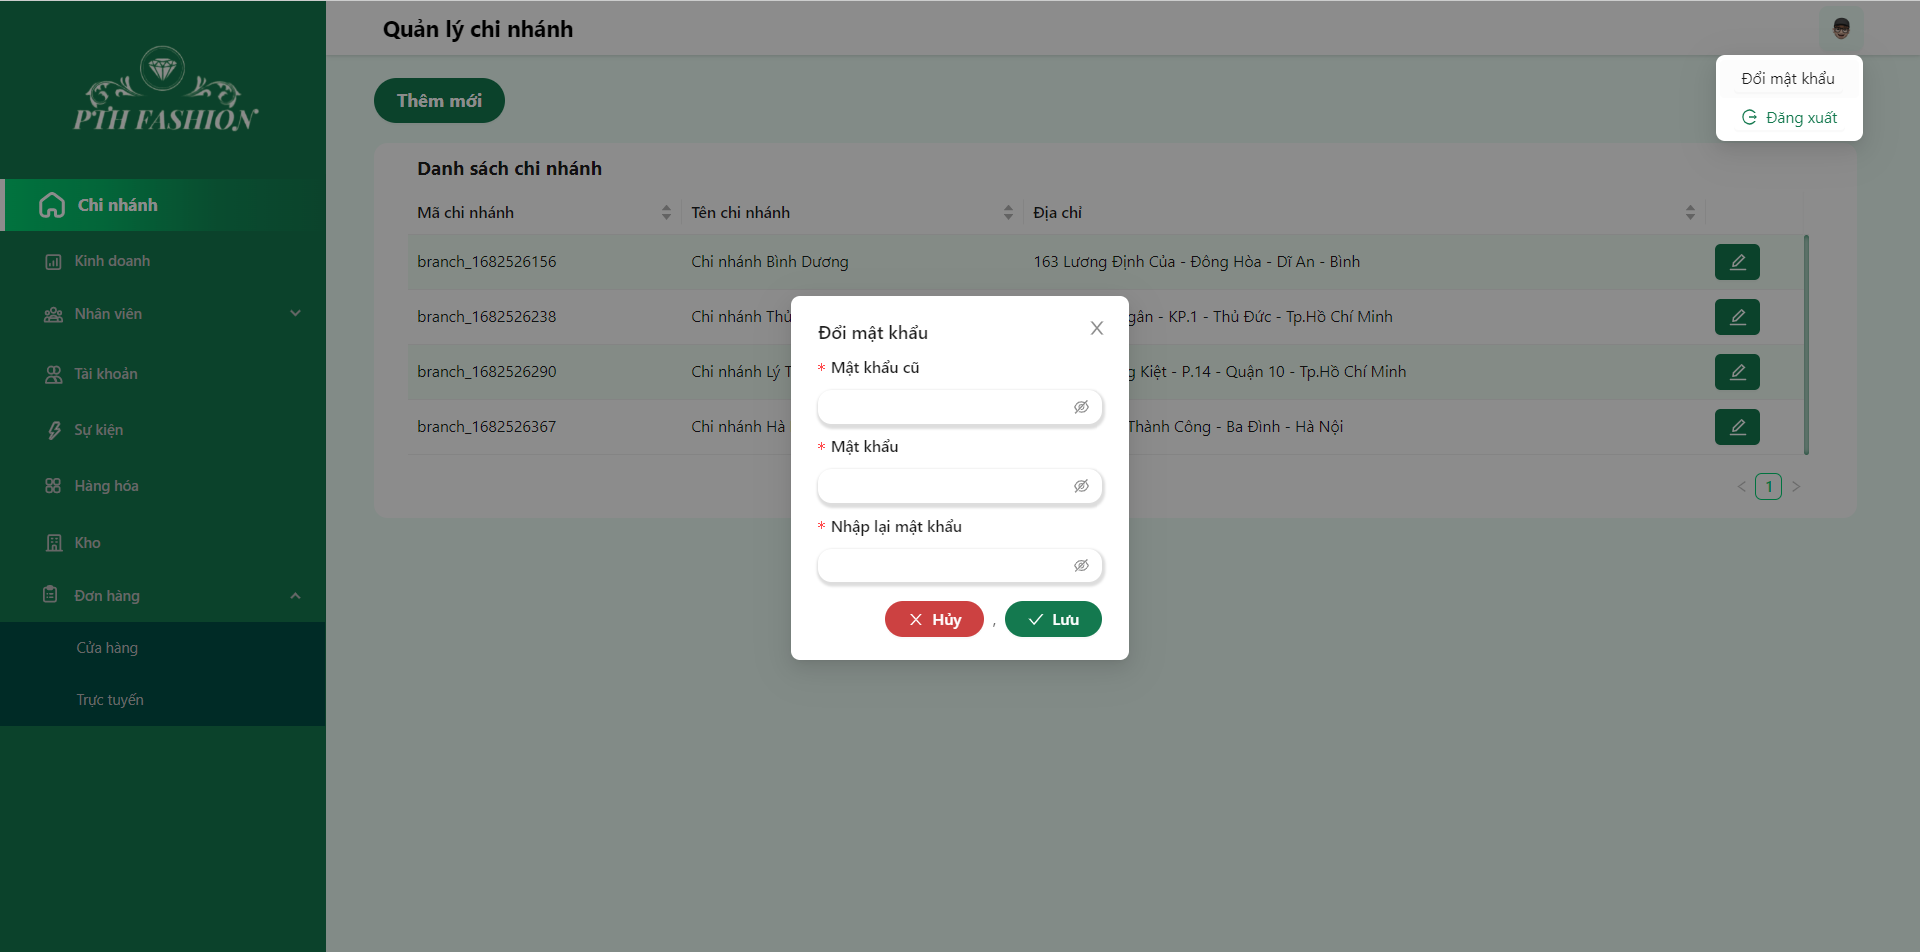
\includegraphics[width=12cm]{img/UI/admin_implement/changePassword.png}
    \label{20}
    \newline
    \caption{Giao diện thay đổi mật khẩu}
\end{figure}


\subsubsection{Quản lý chi nhánh}
\begin{figure}[!htp]
    \centering
    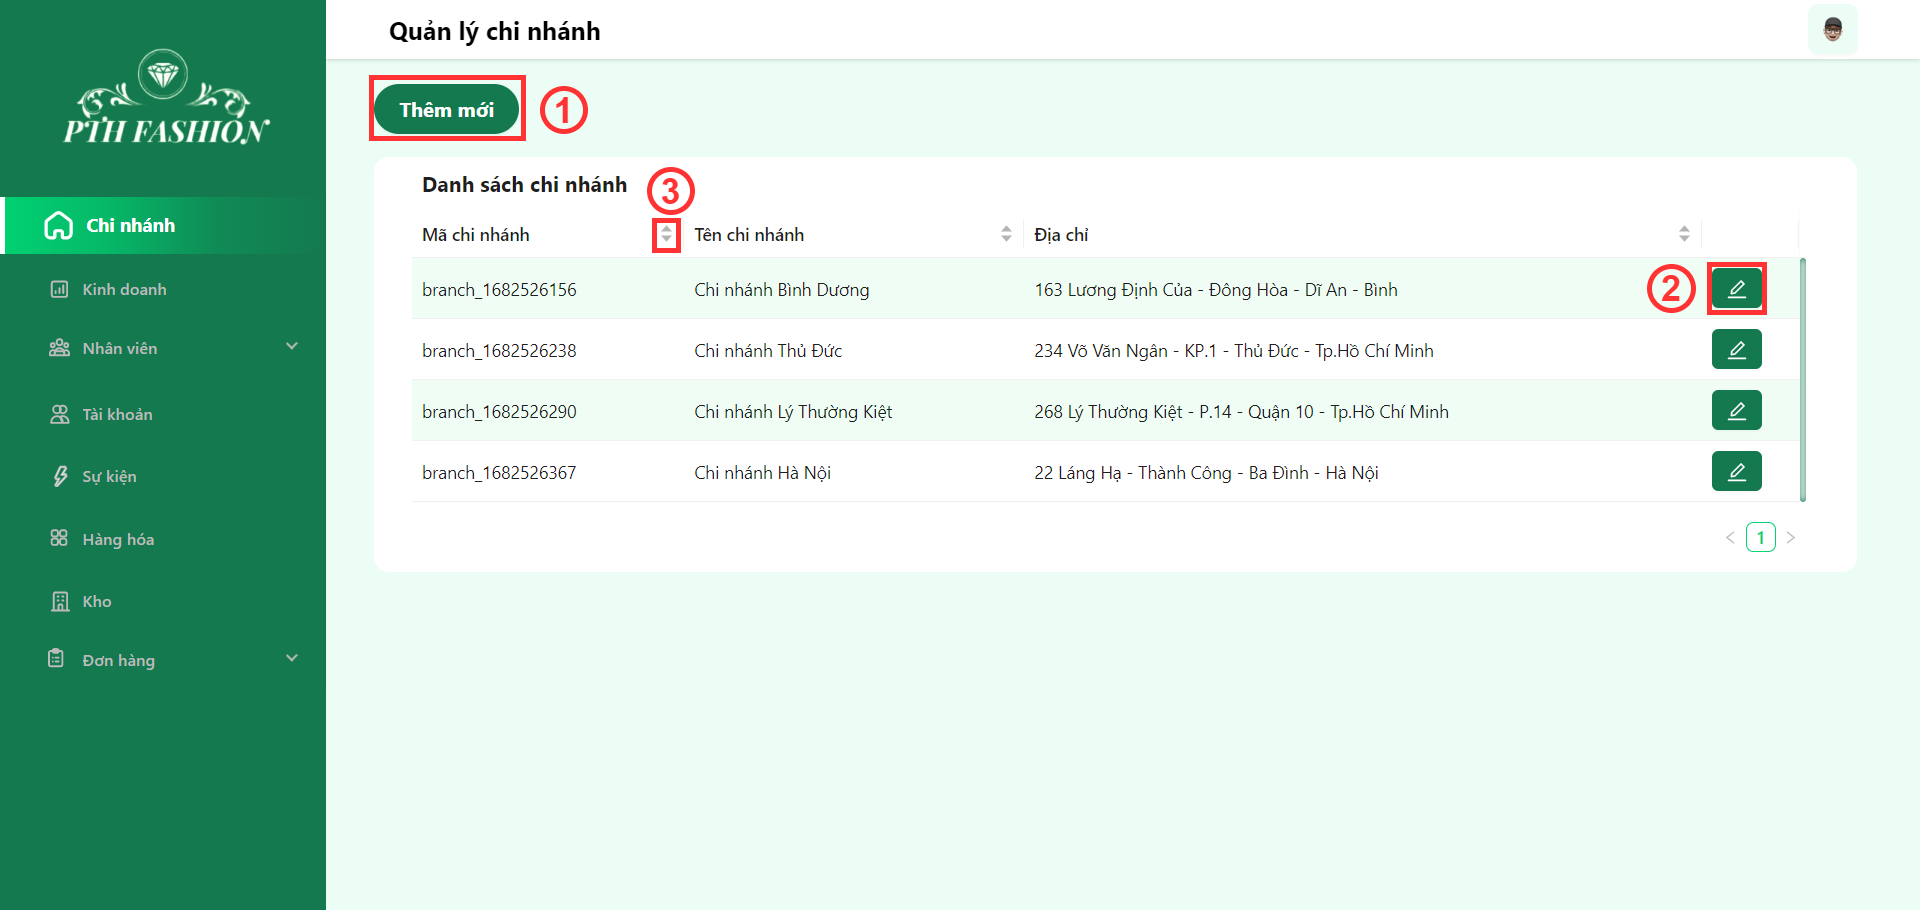
\includegraphics[width=12cm]{img/UI/admin_implement/branch.png}
    \newline
    \caption{Giao diện quản lý chi nhánh}
\end{figure}

\textbf{Mô tả:}
\begin{quote}
    \begin{enumerate}
        \item Chọn để thêm mới chi nhánh
        \item Chọn để chỉnh sửa thông tin chi nhánh
        \item Chọn sắp xếp danh sách chi nhánh theo id
    \end{enumerate}
    Hiển thị danh sách tất cả chi nhánh trong hệ thống. Tương tự cho các tính năng quản lý khác.
\end{quote}

\subsubsubsection{Thông tin chi tiết chi nhánh}
\begin{figure}[!htp]
    \centering
    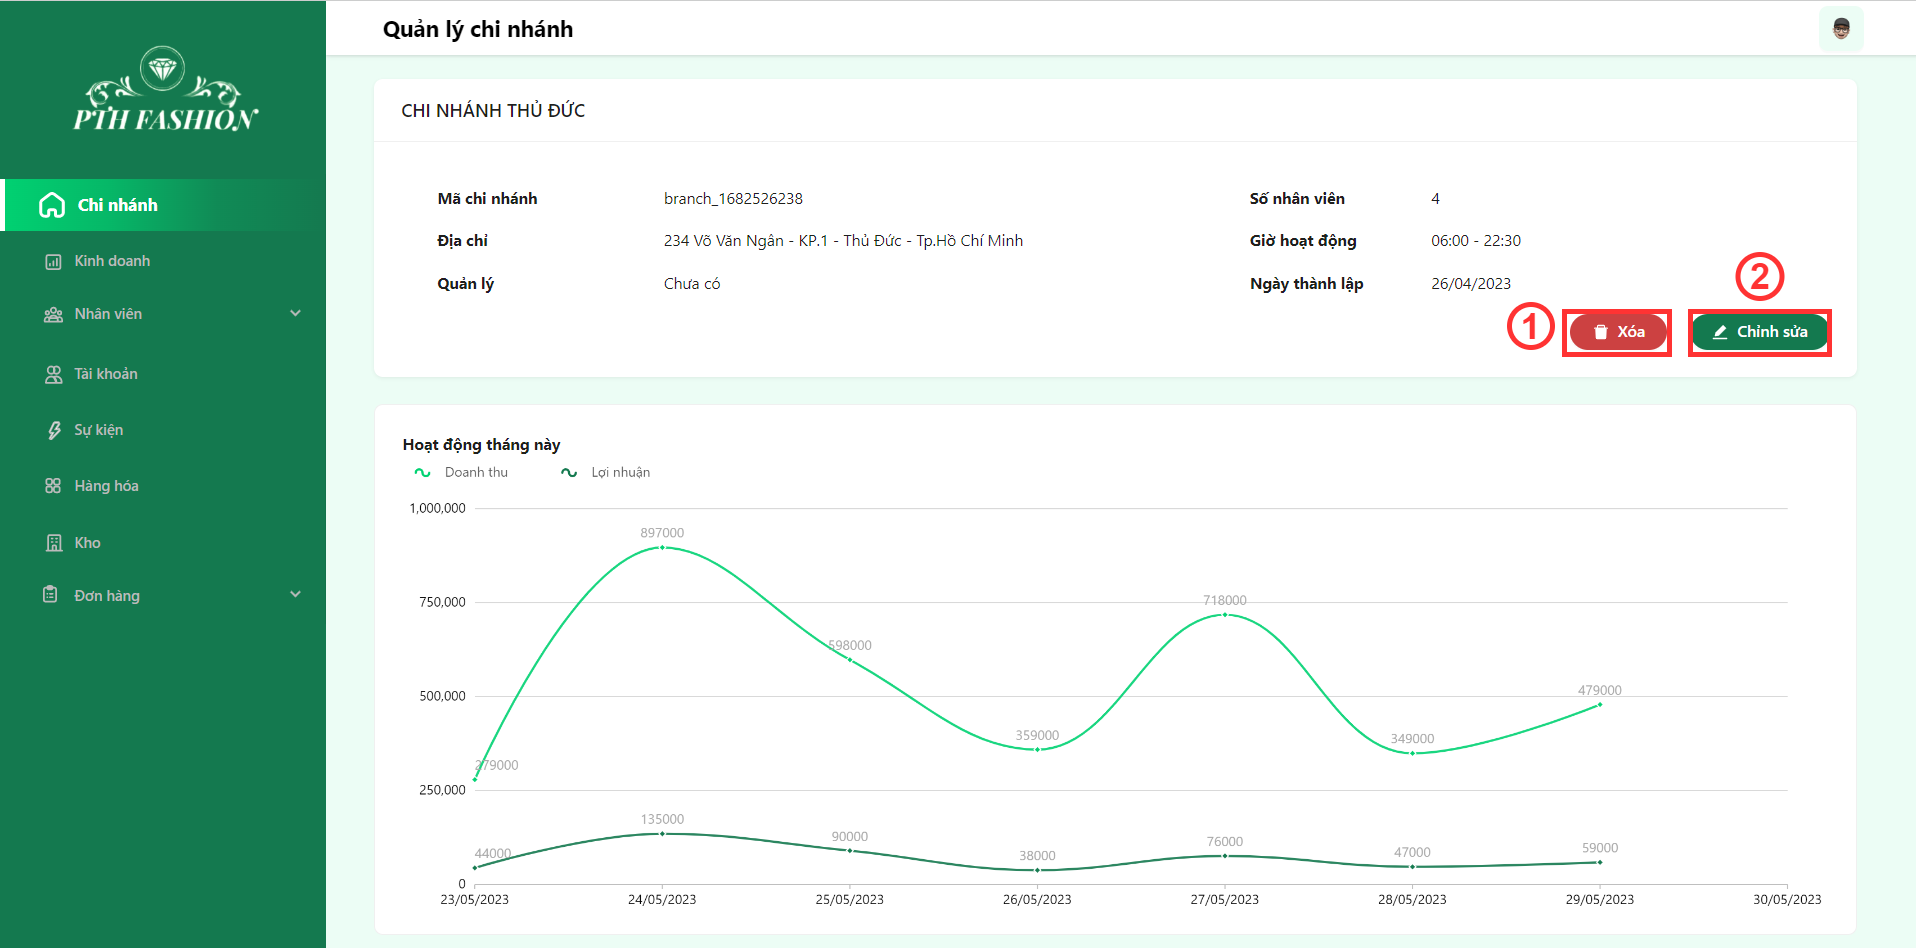
\includegraphics[width=12cm]{img/UI/admin_implement/branchDetail.png}
    \newline
    \caption{Giao diện thông tin chi tiết chi nhánh}
\end{figure}
\textbf{Mô tả:}
\begin{quote}
    \begin{enumerate}
        \item Chọn để xóa chi nhánh
        \item Chọn để hiển thị form "chỉnh sửa chi nhánh"
    \end{enumerate}
    Hiển thị danh sách thông tin chi tiết của chi nhánh. Tương tự cho các tính năng quản lý khác
\end{quote}


\subsubsubsection{Thêm chỉnh sửa chi nhánh}
\begin{figure}[!htp]
    \centering
    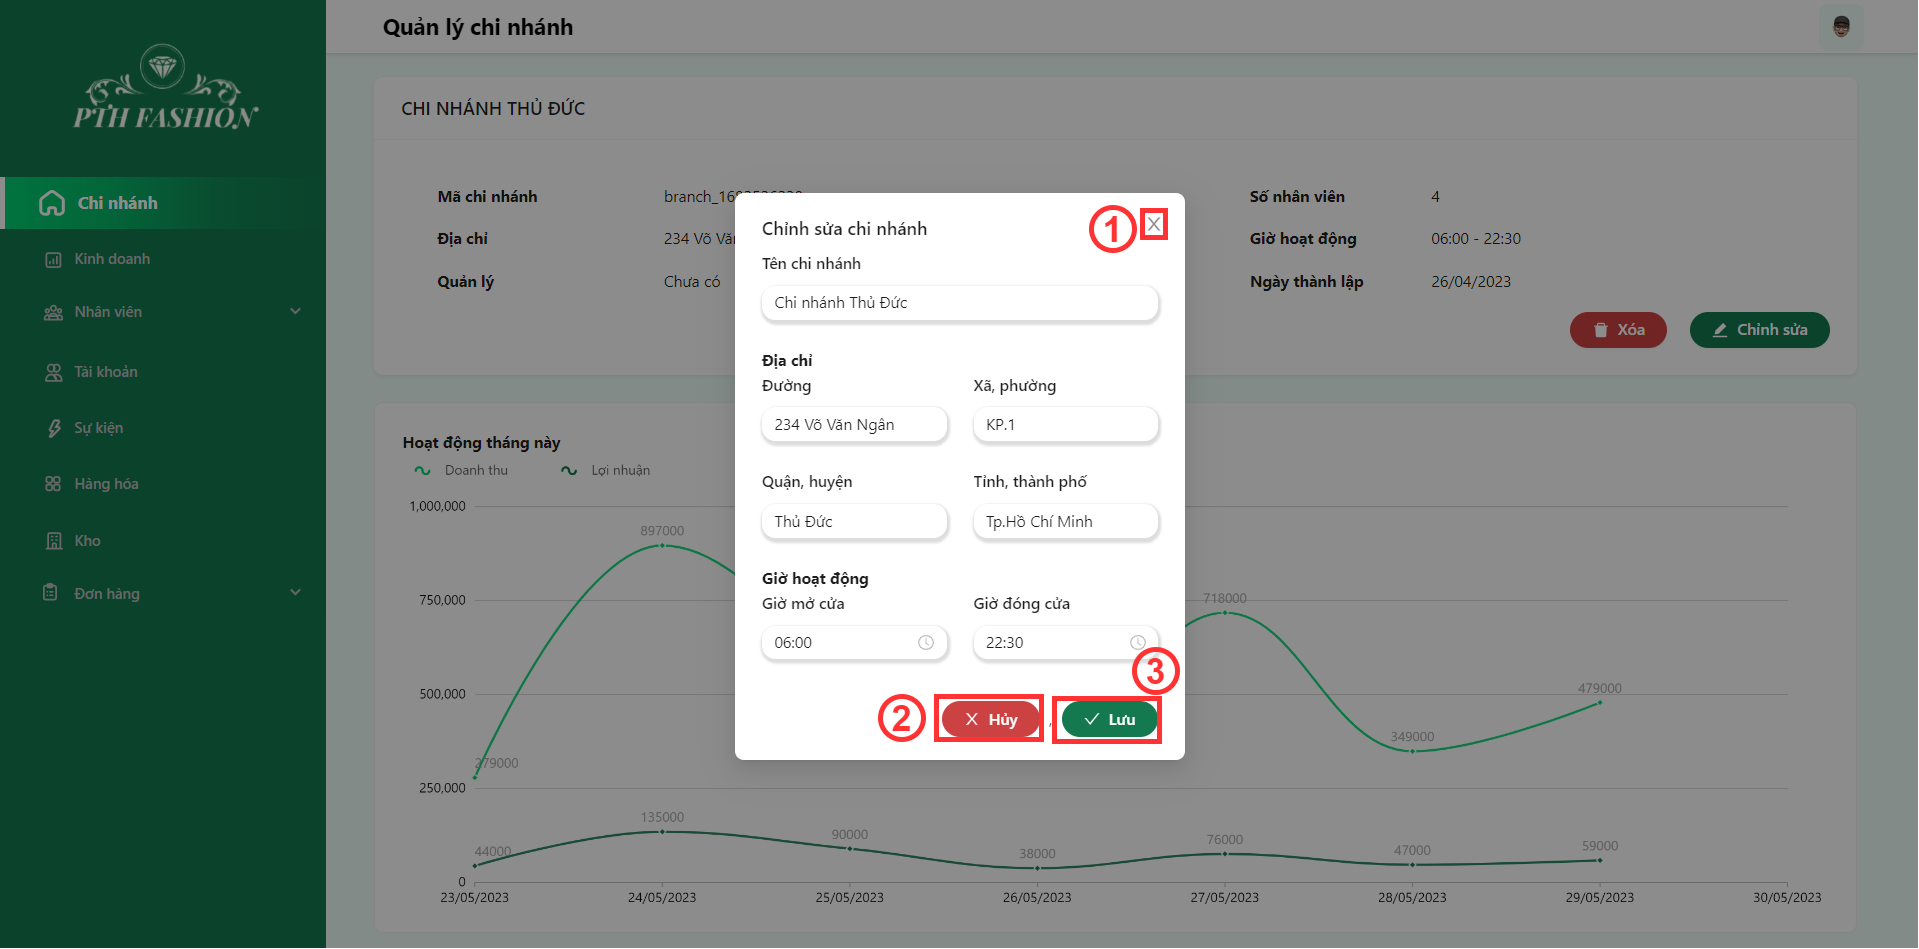
\includegraphics[width=12cm]{img/UI/admin_implement/branchEdit.png}
    \newline
    \caption{Giao diện form thêm mới, chỉnh sửa chi nhánh}
\end{figure}
\textbf{Mô tả:}
\begin{quote}
    \begin{enumerate}
        \item Chọn để hủy thay đổi
        \item Chọn để hủy thay đổi
        \item Chọn để lưu thay đổi
    \end{enumerate}
    Nhập các thông tin để thêm mới hoặc chỉnh sửa chi nhánh. Tương tự cho các tính năng quản lý khác
\end{quote}

\newpage

\subsubsection{Quản lý hoạt động kinh doanh}
\begin{figure}[!htp]
    \centering
    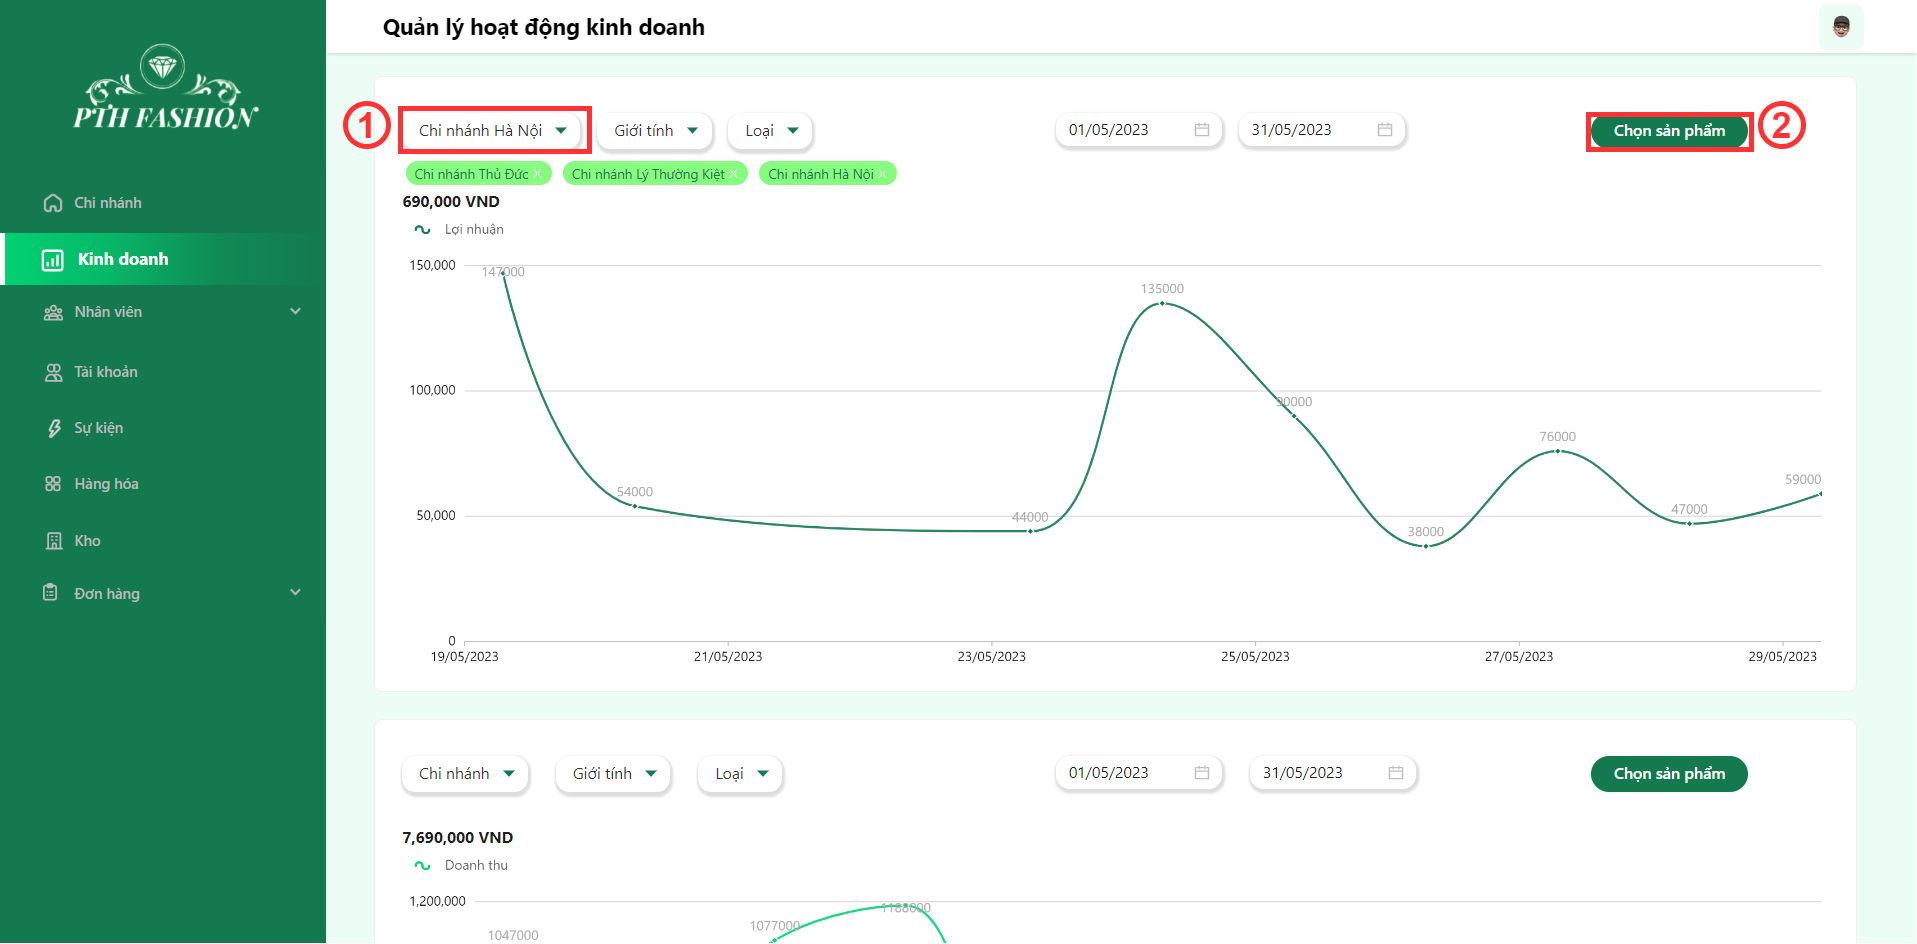
\includegraphics[width=12cm]{img/UI/admin_implement/statistic.png}
    \newline
    \caption{Giao diện quản lý hoạt động kinh doanh}
\end{figure}
\textbf{Mô tả:}
\begin{quote}
    \begin{enumerate}
        \item Chọn để lọc thống kê theo chi nhánh, tương tự với các tính năng lọc còn lại
        \item Chọn một sản phẩm để thống kê
    \end{enumerate}
\end{quote}


\subsubsection{Quản lý nhân viên}
\begin{figure}[!htp]
    \centering
    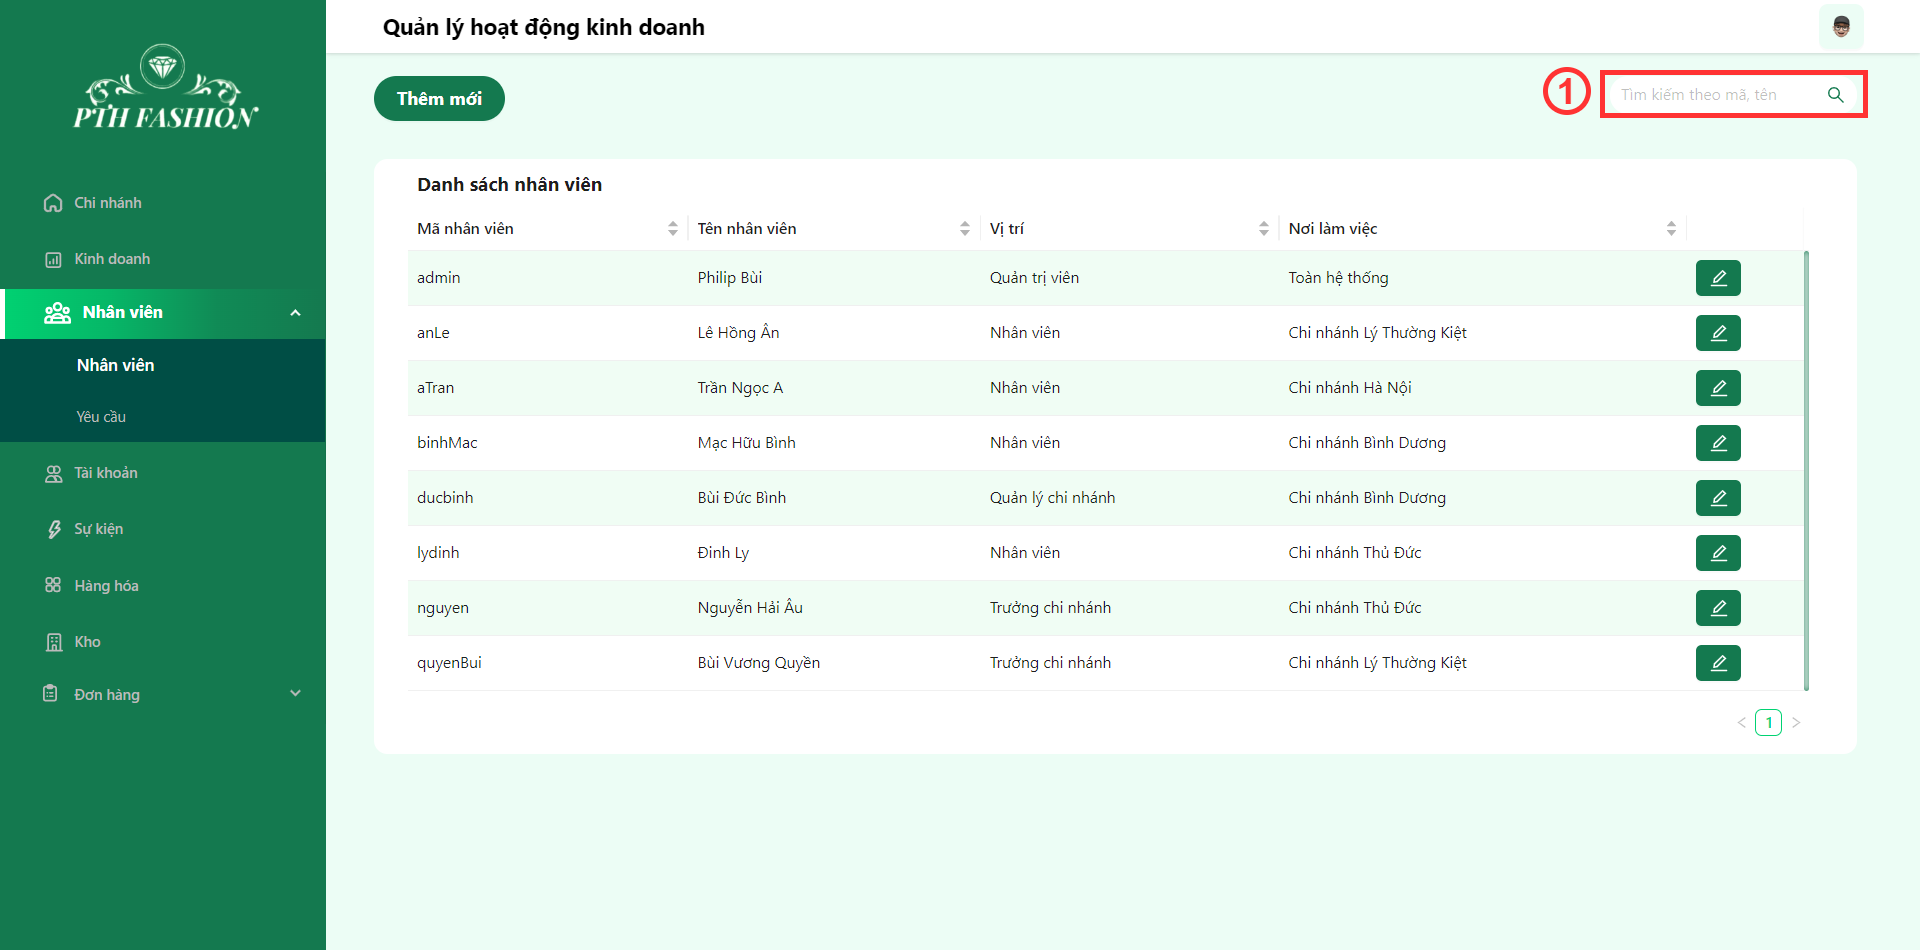
\includegraphics[width=12cm]{img/UI/admin_implement/staff.png}
    \newline
    \caption{Giao diện quản lý nhân viên}
\end{figure}
\textbf{Mô tả:}
\begin{quote}
    \begin{enumerate}
        \item Nhập để tìm kiếm nhân viên theo mã, tên
    \end{enumerate}
    Hiển thị danh sách tất cả nhân viên trong hệ thống. chức năng tìm kiếm tương tự cho các tính năng quản lý khác.
\end{quote}


\newpage

\subsubsubsection{Thêm, chỉnh sửa nhân viên}
\begin{figure}[!htp]
    \centering
    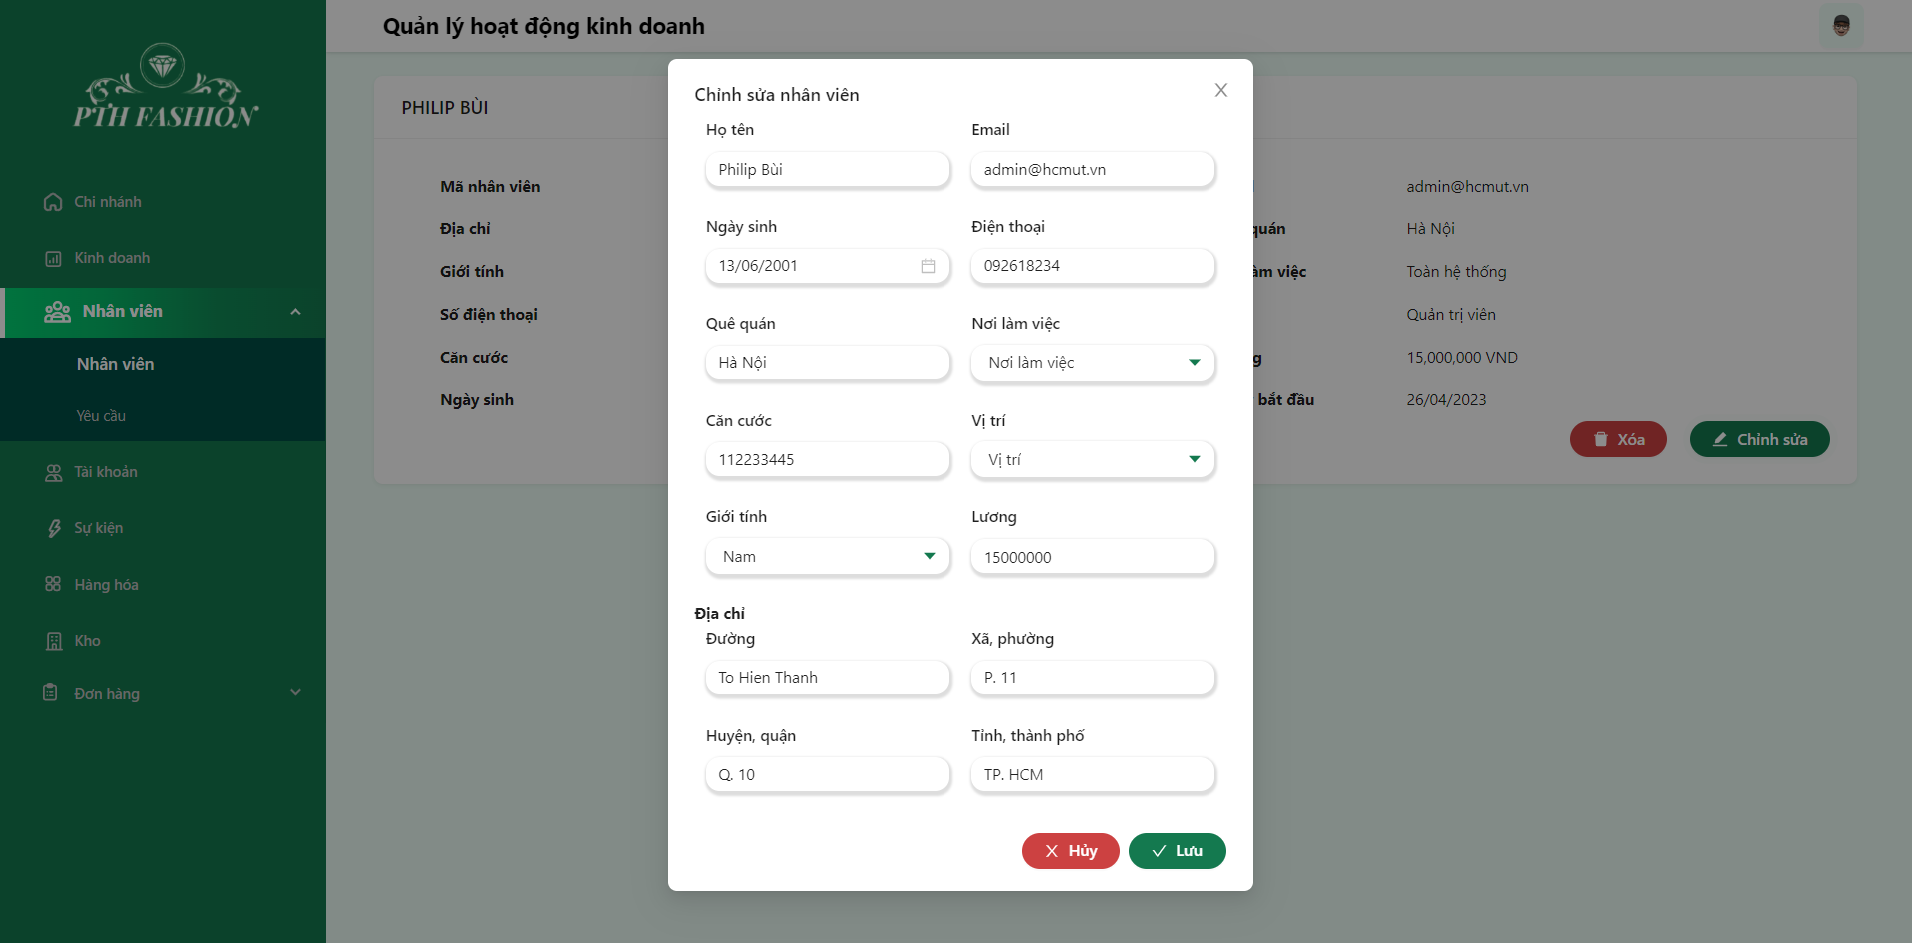
\includegraphics[width=12cm]{img/UI/admin_implement/staffEdit.png}
    \newline
    \caption{Form thêm, chỉnh sửa nhân viên}
\end{figure}


\subsubsubsection{Thông tin chi tiết nhân viên}
\begin{figure}[!htp]
    \centering
    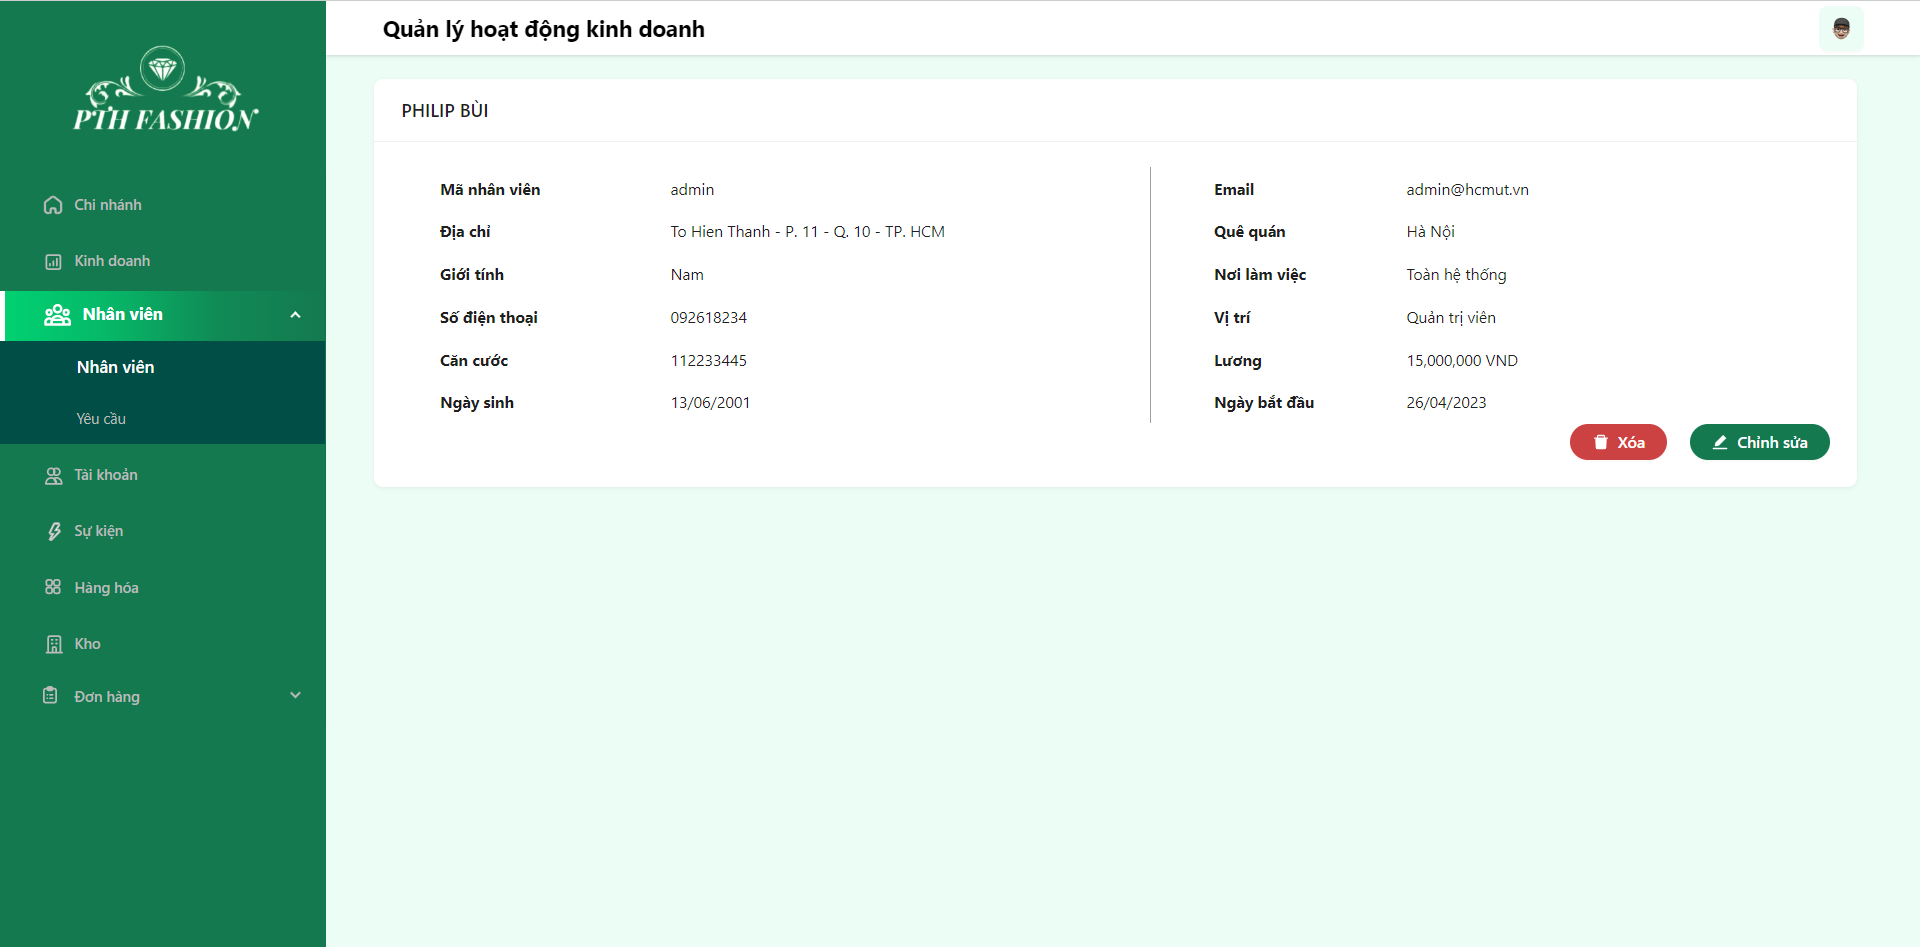
\includegraphics[width=12cm]{img/UI/admin_implement/staffDetail.png}
    \newline
    \caption{Giao diện thông tin chi tiết nhân viên}
\end{figure}


\newpage

\subsubsubsection{Quản lý yêu cầu nhân viên}
\begin{figure}[!htp]
    \centering
    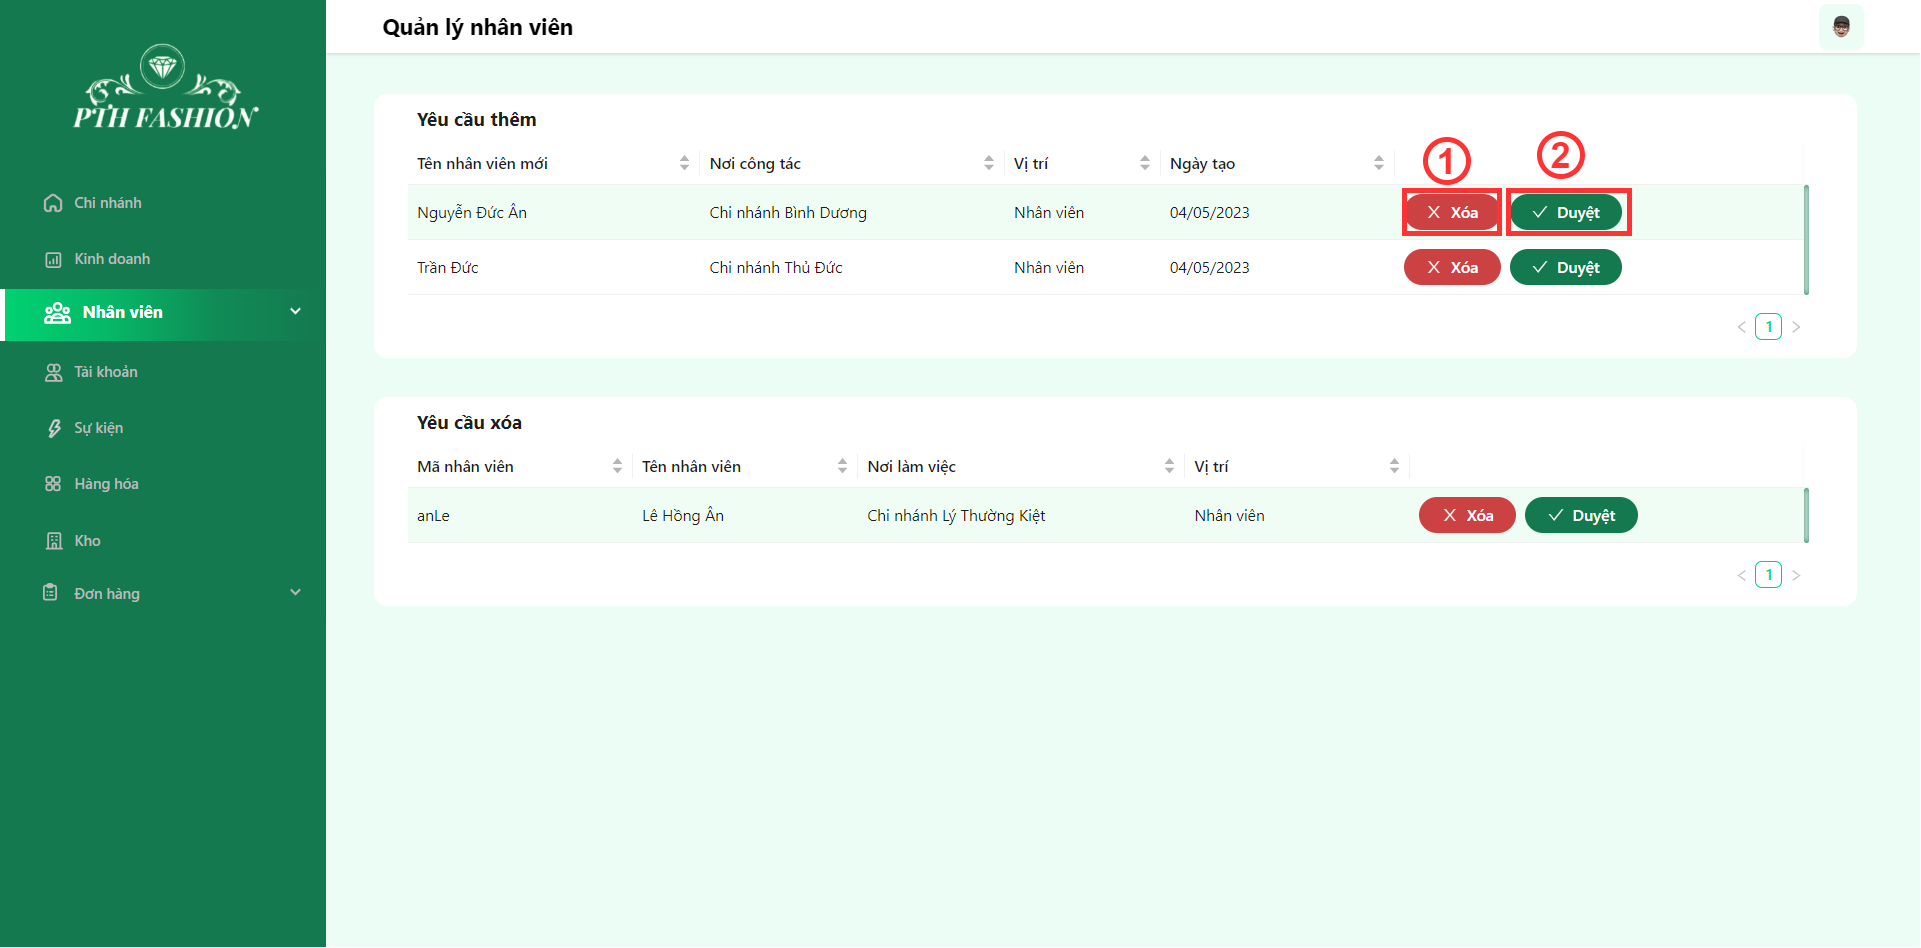
\includegraphics[width=12cm]{img/UI/admin_implement/staffRequest.png}
    \newline
    \caption{Giao diện quản lý yêu cầu nhân viên}
\end{figure}
\textbf{Mô tả:}
\begin{quote}
    \begin{enumerate}
        \item Chọn để xóa yêu cầu
        \item Chọn để duyệt yêu cầu
    \end{enumerate}
\end{quote}

\subsubsubsection{Thông tin chi tiết của yêu cầu nhân viên}
\begin{figure}[!htp]
    \centering
    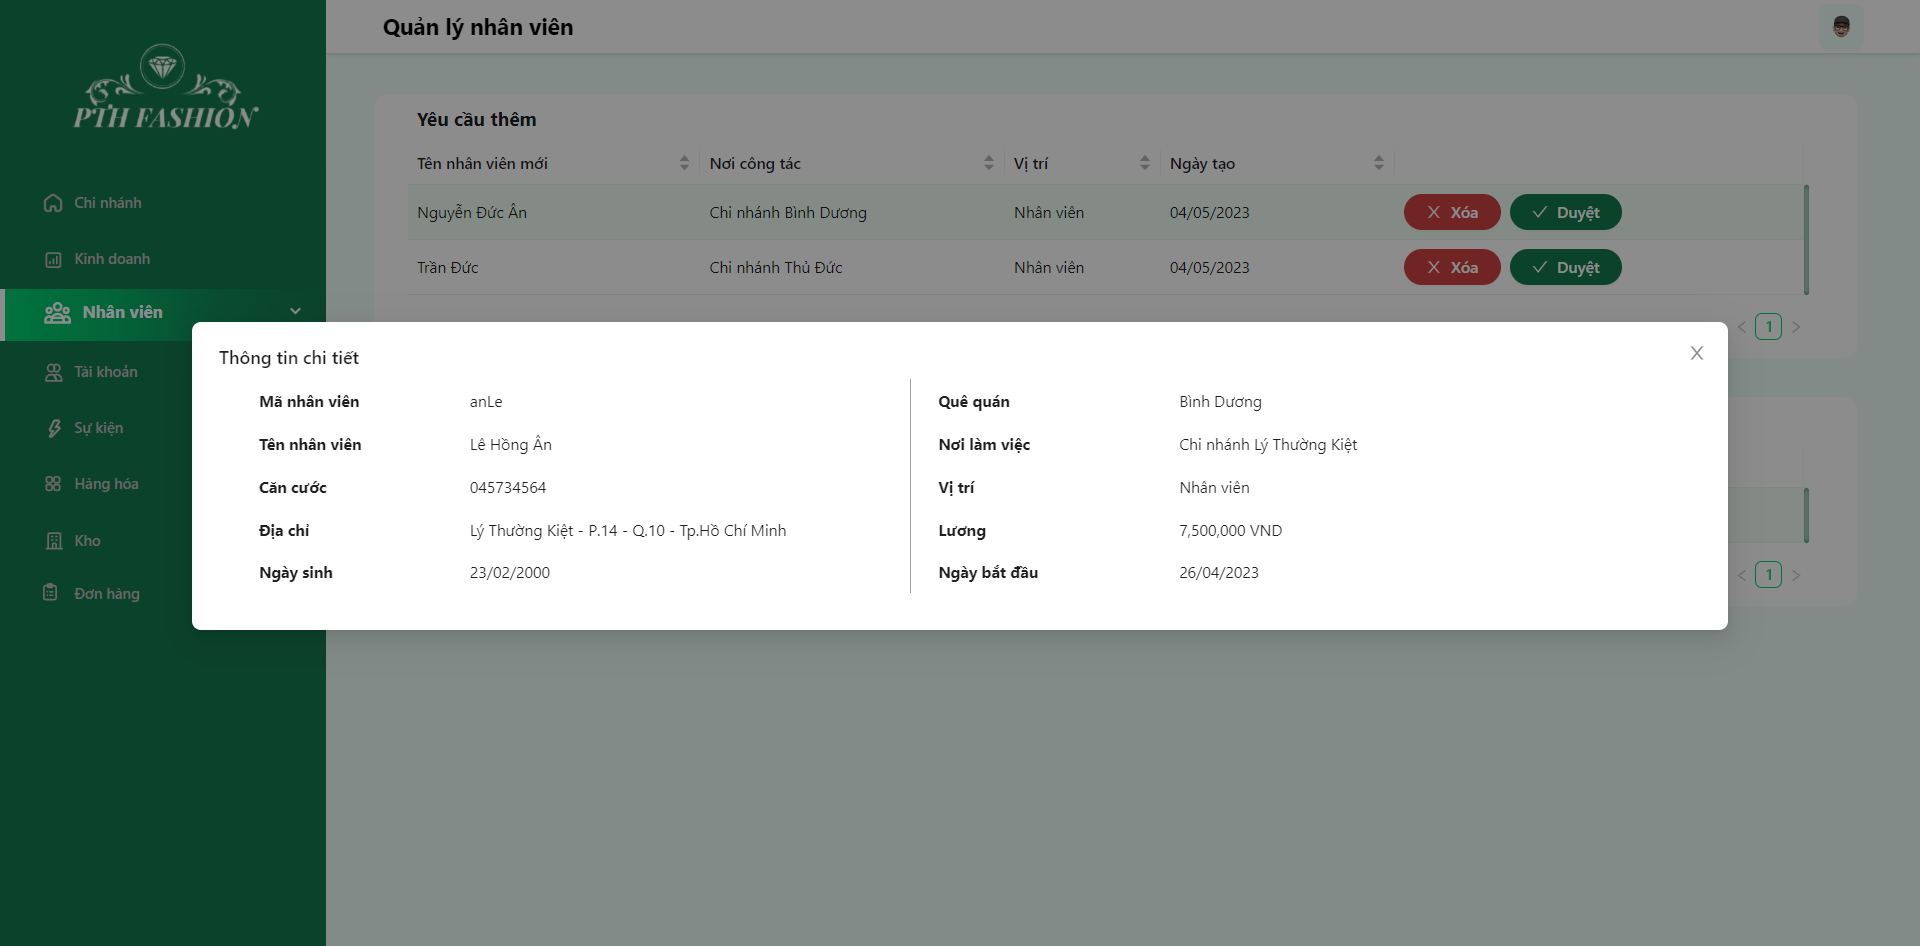
\includegraphics[width=12cm]{img/UI/admin_implement/staffRequestDetail.png}
    \newline
    \caption{Giao diện Thông tin chi tiết của yêu cầu nhân viên}
\end{figure}

% \subsubsubsection{Yêu cầu thêm nhân viên}
% \subsubsubsection{Yêu cầu xóa nhân viên}

\newpage

\subsubsection{Quản lý tài khoản}
\begin{figure}[!htp]
    \centering
    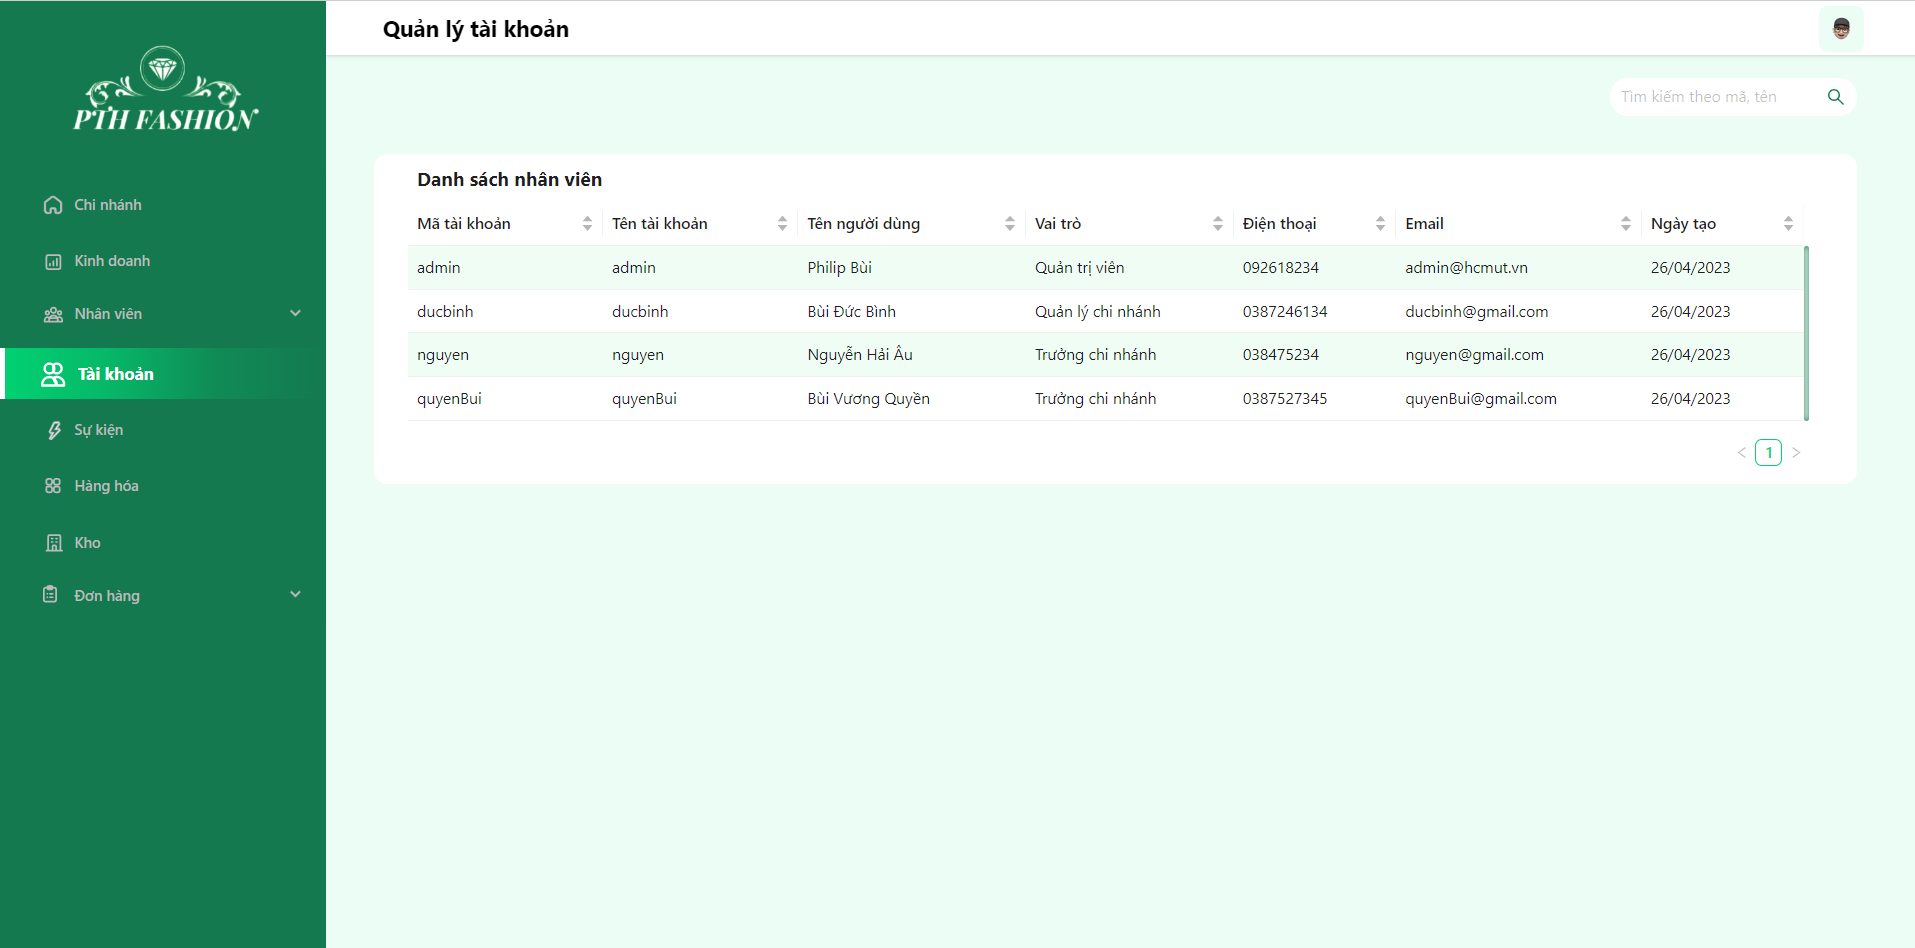
\includegraphics[width=12cm]{img/UI/admin_implement/account.png}
    \newline
    \caption{Giao diện quản lý tài khoản}
\end{figure}


\subsubsection{Quản lý kho}
\begin{figure}[!htp]
    \centering
    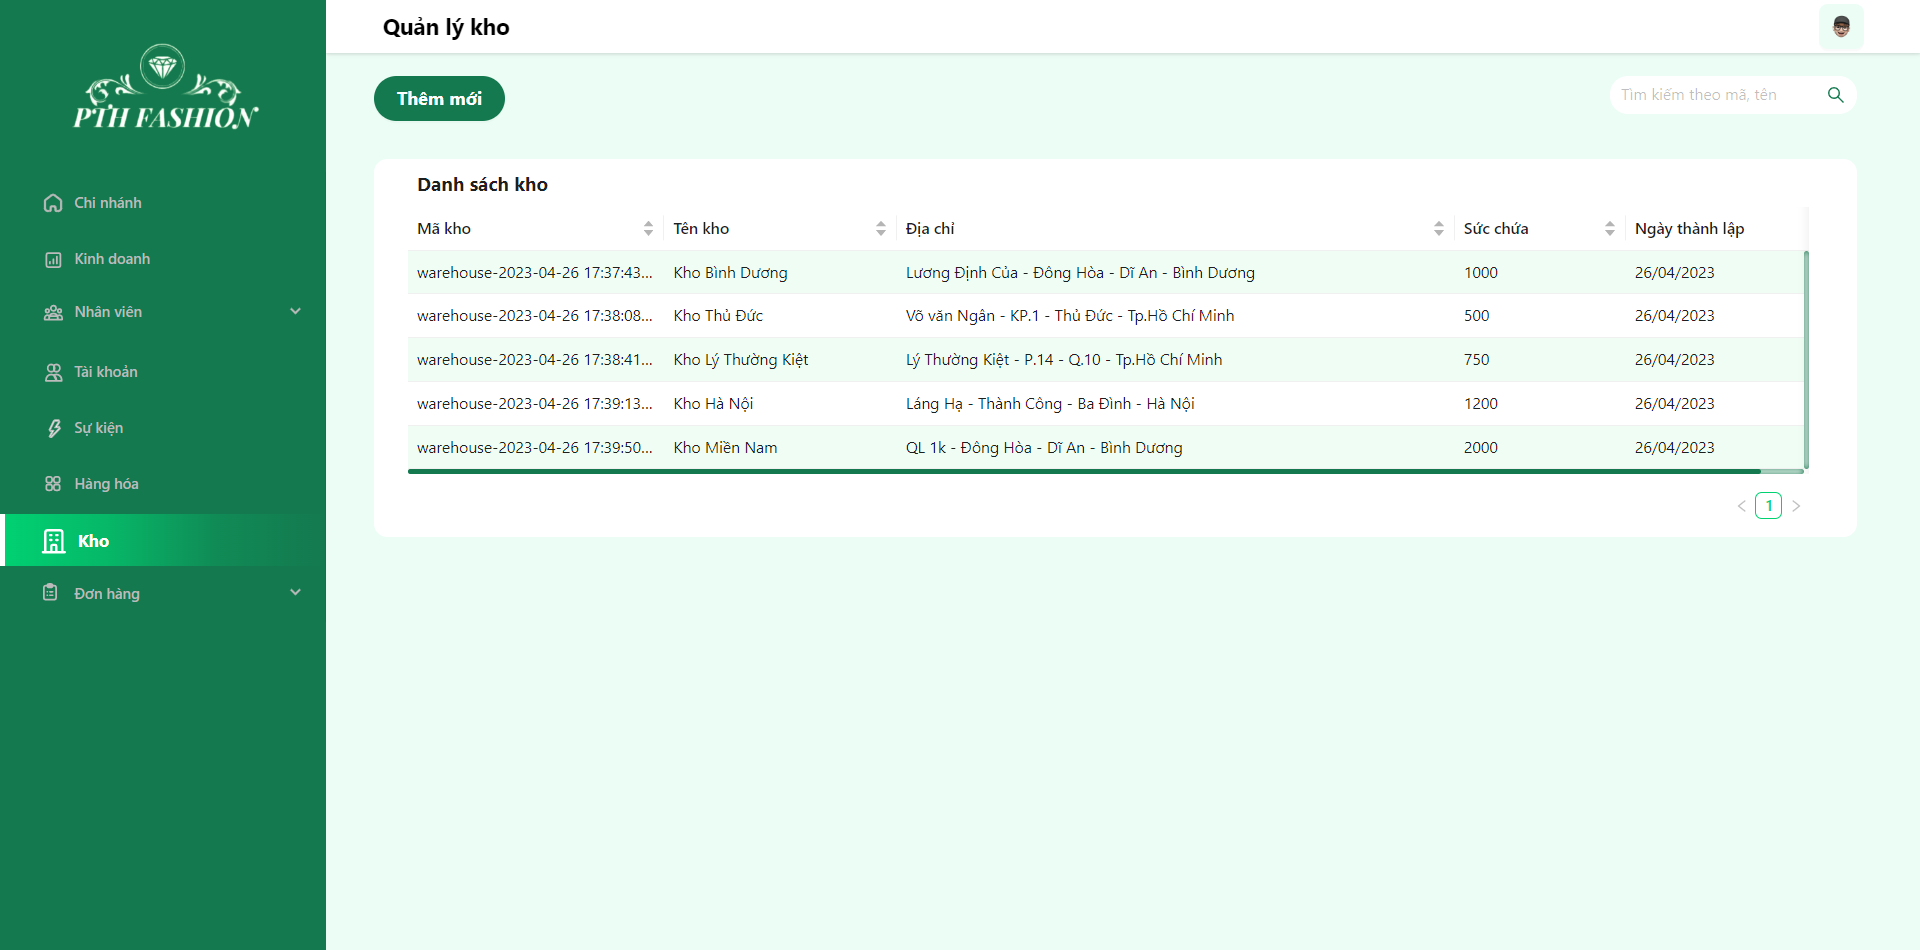
\includegraphics[width=12cm]{img/UI/admin_implement/warehouse.png}
    \newline
    \caption{Giao diện quản lý kho}
\end{figure}


\newpage

\subsubsubsection{Thêm, chỉnh sửa thông tin kho}
\begin{figure}[!htp]
    \centering
    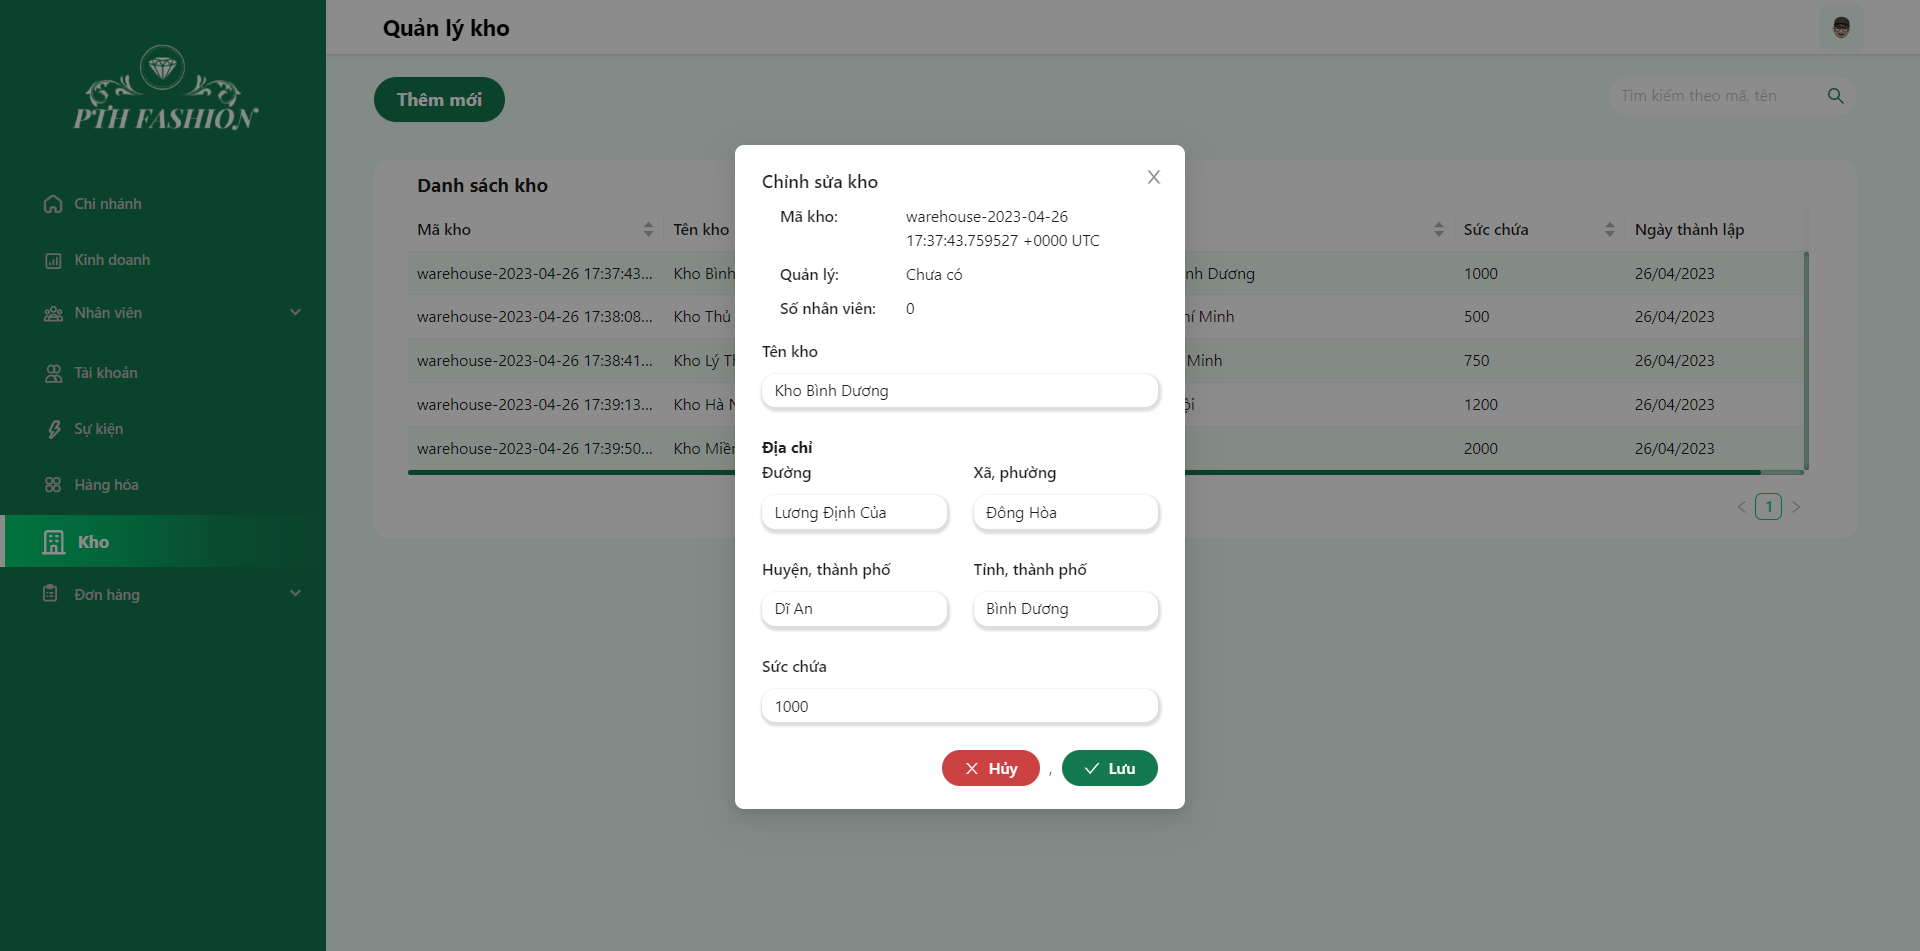
\includegraphics[width=12cm]{img/UI/admin_implement/warehouseEdit.png}
    \newline
    \caption{Giao diện thêm, chỉnh sửa thông tin kho}
\end{figure}





\subsubsection{Quản lý sự kiện}
\begin{figure}[!htp]
    \centering
    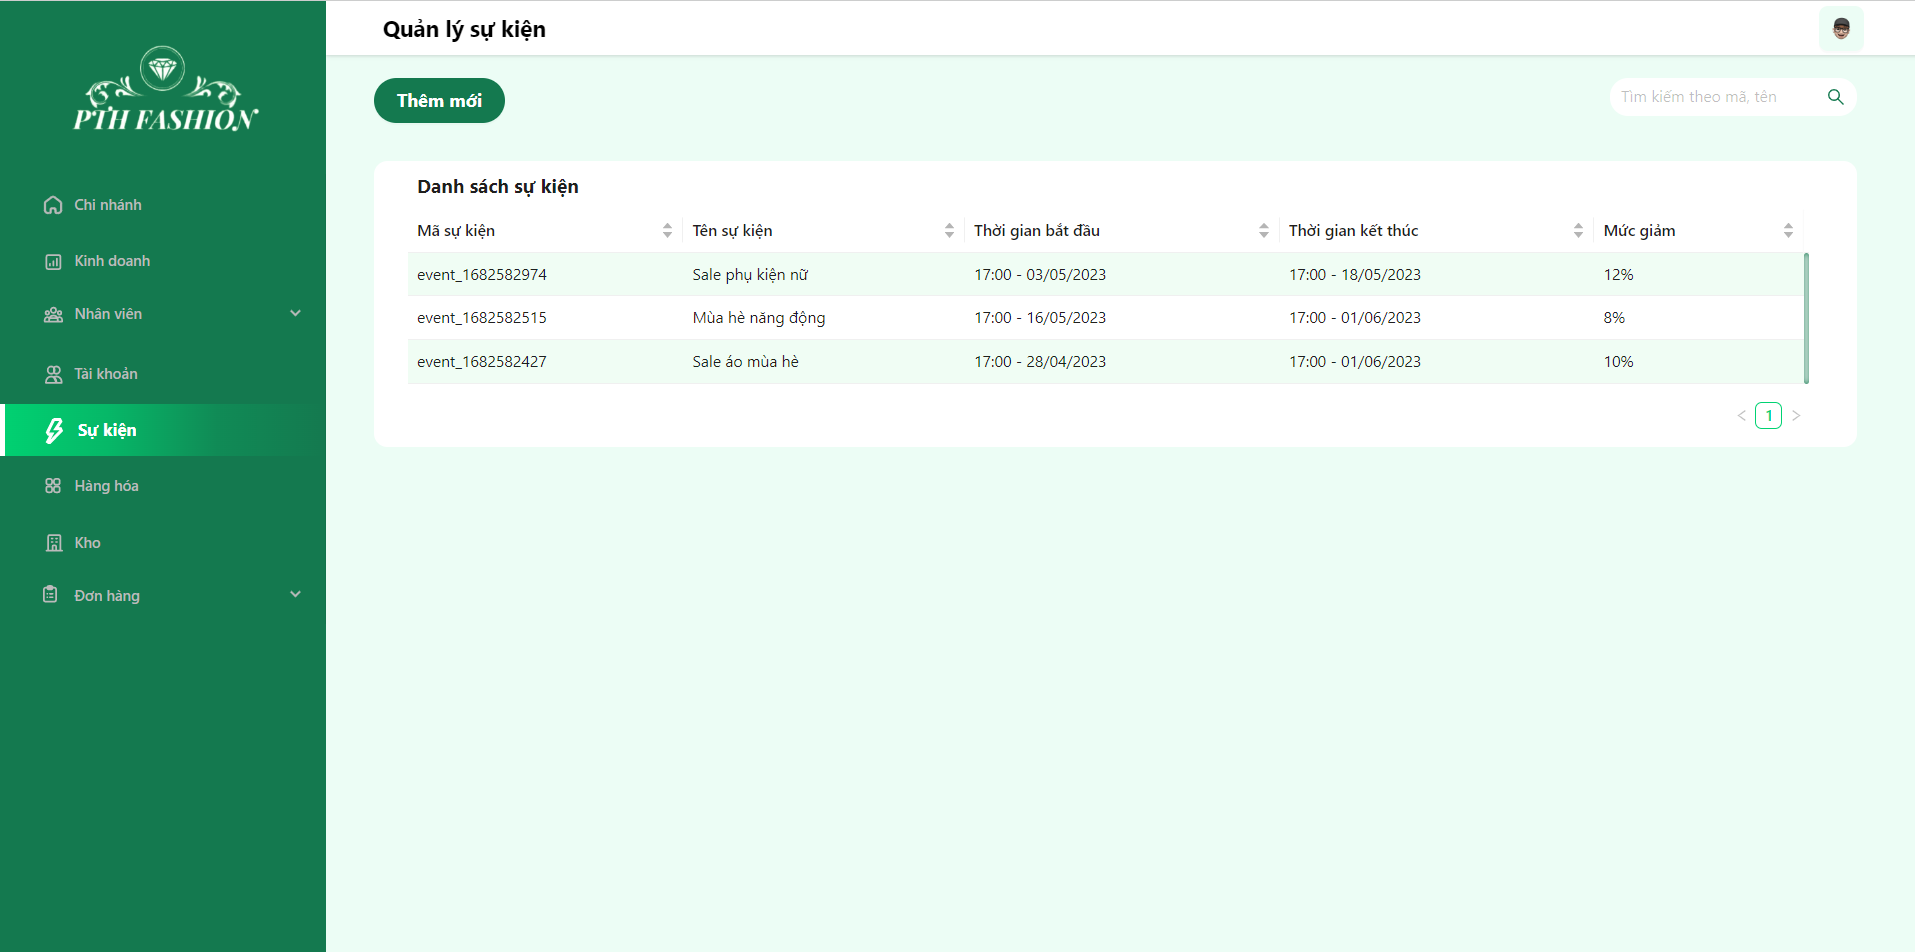
\includegraphics[width=12cm]{img/UI/admin_implement/event.png}
    \newline
    \caption{Giao diện quản lý sự kiện}
\end{figure}


\newpage

\subsubsubsection{Thêm, chỉnh sửa thông tin sự kiện}
\begin{figure}[!htp]
    \centering
    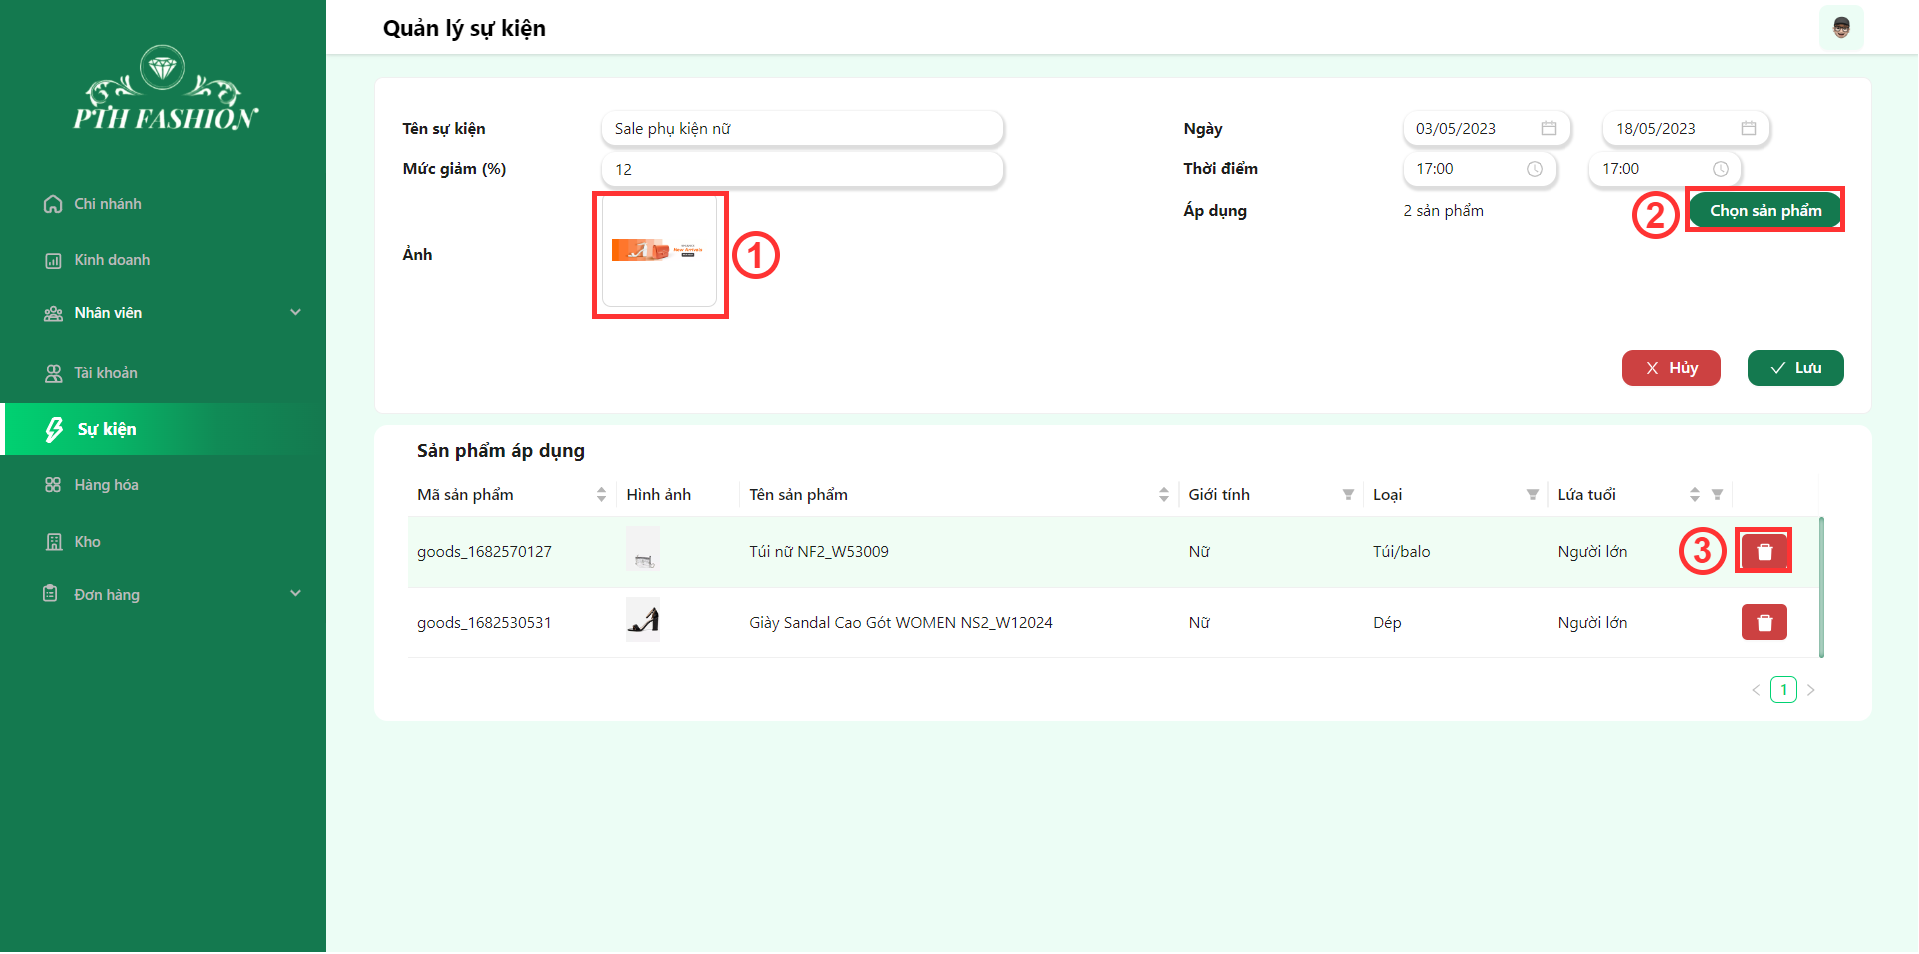
\includegraphics[width=12cm]{img/UI/admin_implement/eventEdit.png}
    \newline
    \caption{Giao diện thêm, chỉnh sửa thông tin sự kiện}
\end{figure}
\textbf{Mô tả:}
\begin{quote}
    \begin{enumerate}
        \item Chọn để tải ảnh lên cho sự kiện
        \item Chọn để chọn danh sách hàng cho sự kiện
        \item Chọn xóa hàng khỏi sự kiện
    \end{enumerate}
\end{quote}

% \newpage

\subsubsubsection{Chọn hàng cho sự kiện}
\begin{figure}[!htp]
    \centering
    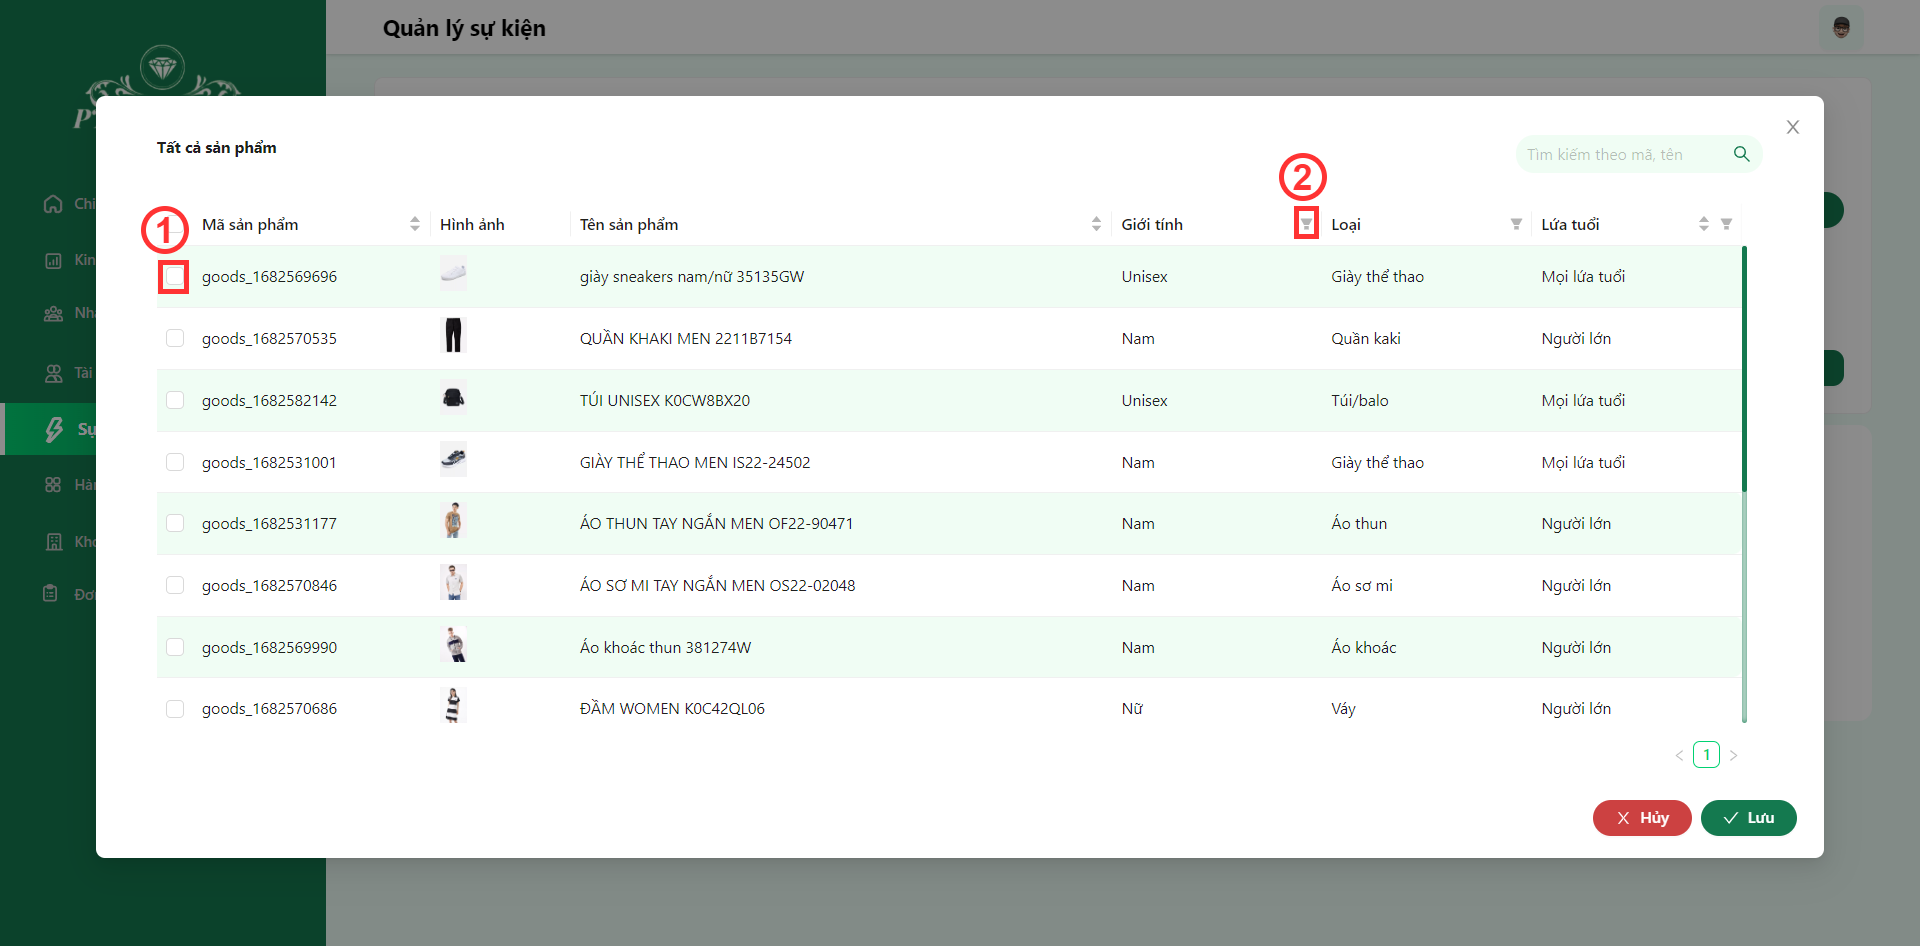
\includegraphics[width=12cm]{img/UI/admin_implement/eventAllGoods.png}
    \newline
    \caption{Giao diện chọn hàng cho sự kiện}
\end{figure}
\textbf{Mô tả:}
\begin{quote}
    \begin{enumerate}
        \item Chọn để thêm hàng cho sự kiện
        \item Chọn để lọc hàng theo loại hàng, tương tự các tính năng lọc khác
    \end{enumerate}
\end{quote}

\newpage
\subsubsection{Quản lý hàng hóa}
\begin{figure}[!htp]
    \centering
    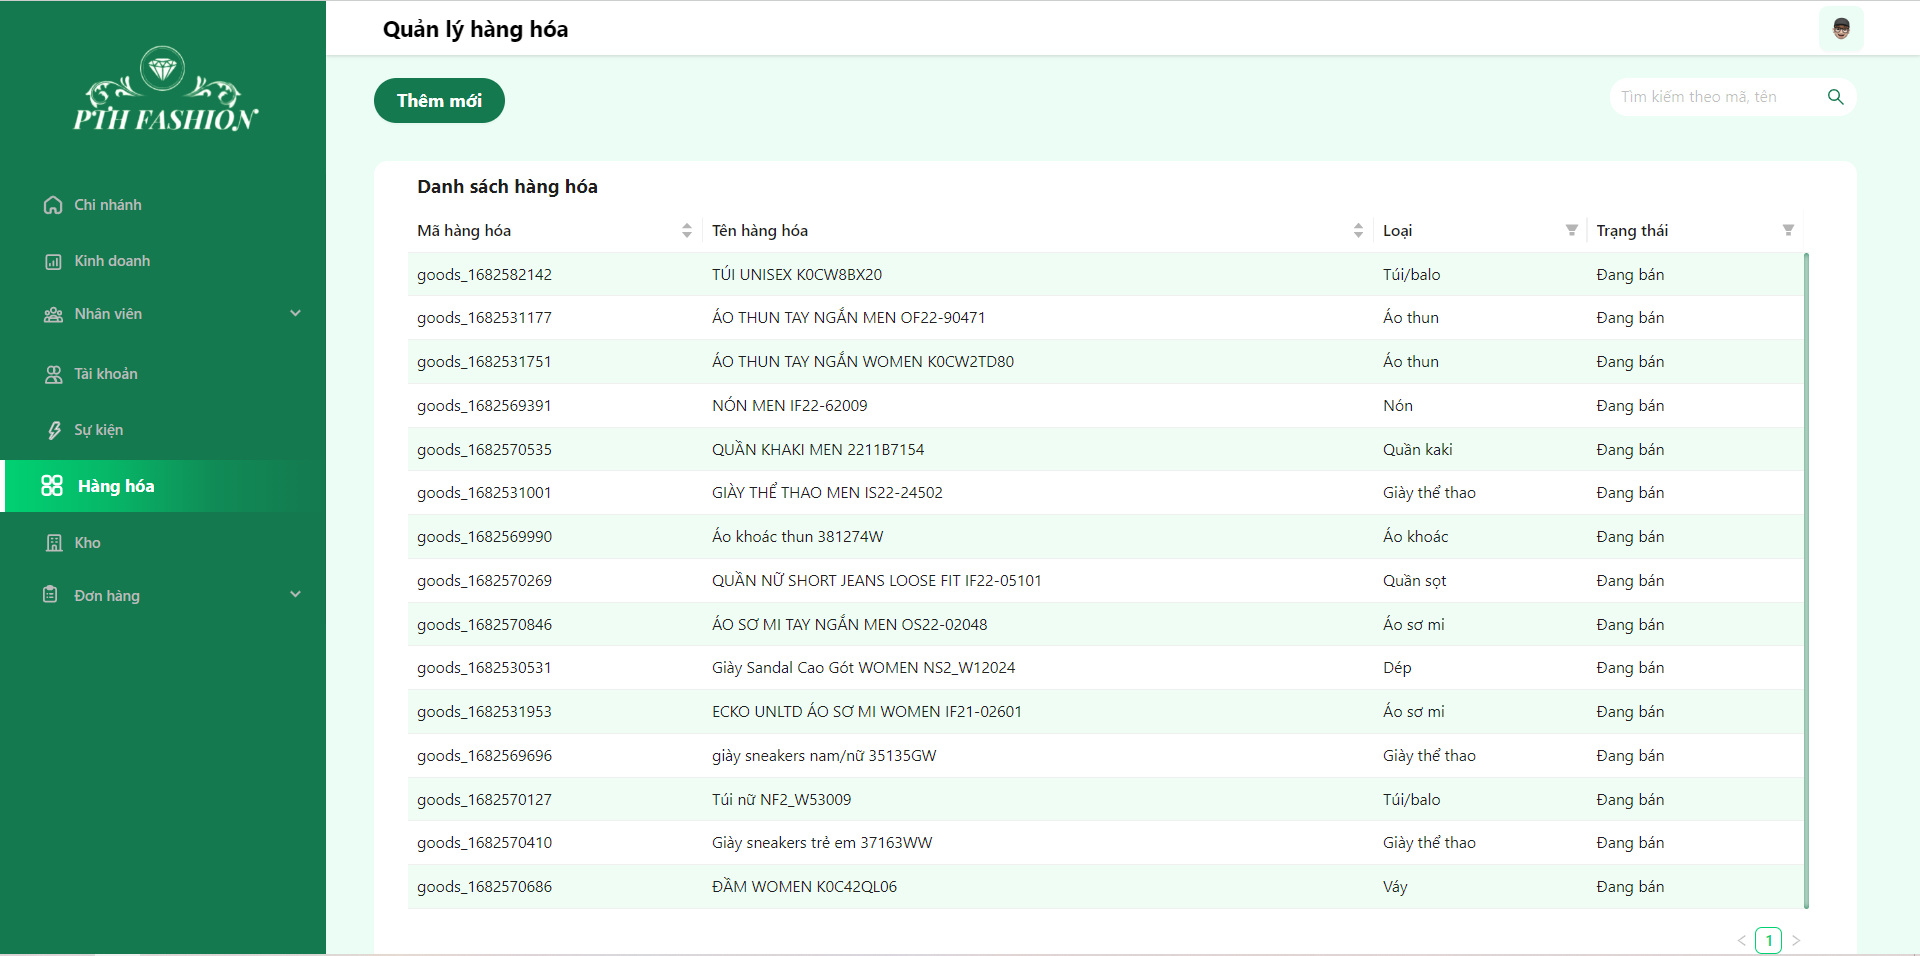
\includegraphics[width=12cm]{img/UI/admin_implement/goods.png}
    \newline
    \caption{Giao diện quản lý hàng hóa}
\end{figure}


\subsubsubsection{Thêm, chỉnh sửa thông tin hàng}
\begin{figure}[!htp]
    \centering
    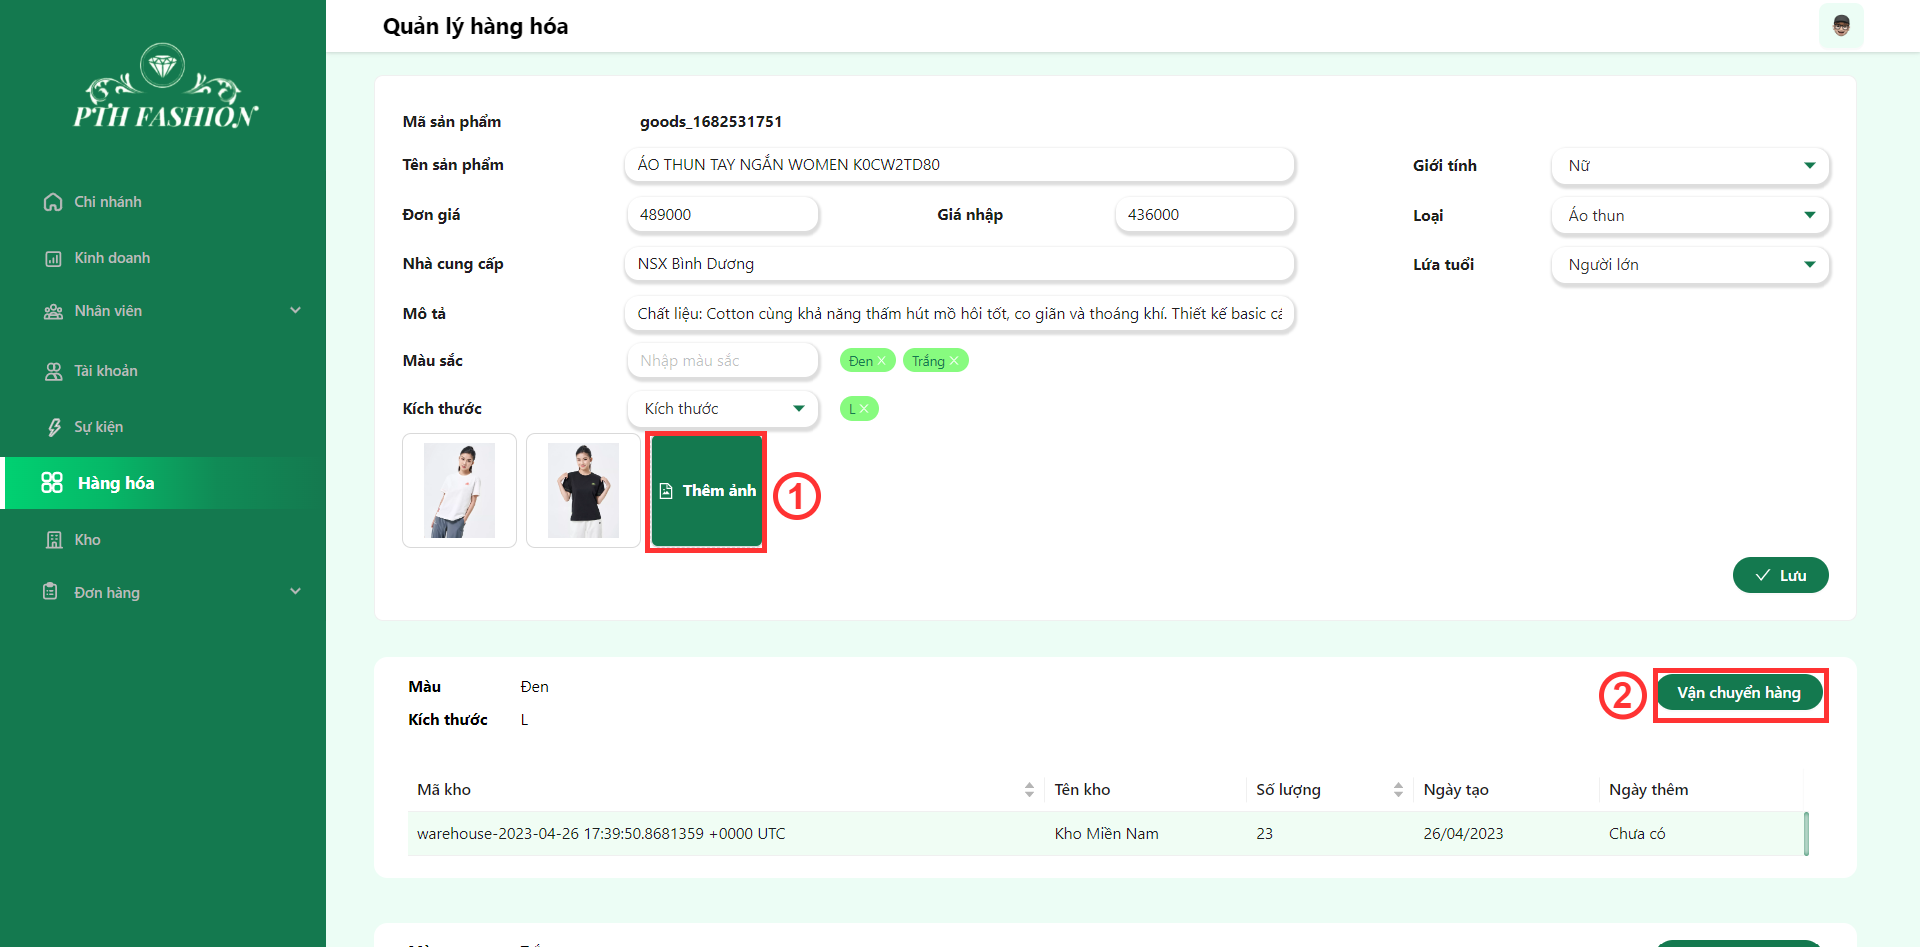
\includegraphics[width=12cm]{img/UI/admin_implement/goodsEdit.png}
    \newline
    \caption{Giao diện thêm mới, chỉnh sửa thông tin hàng}
\end{figure}
\textbf{Mô tả:}
\begin{quote}
    \begin{enumerate}
        \item Chọn để mở modal thêm ảnh cho hàng
        \item Chọn để mở modal vận chuyển hàng hàng
    \end{enumerate}
\end{quote}


\newpage
\subsubsubsection{Thêm ảnh cho hàng hàng}
\begin{figure}[!htp]
    \centering
    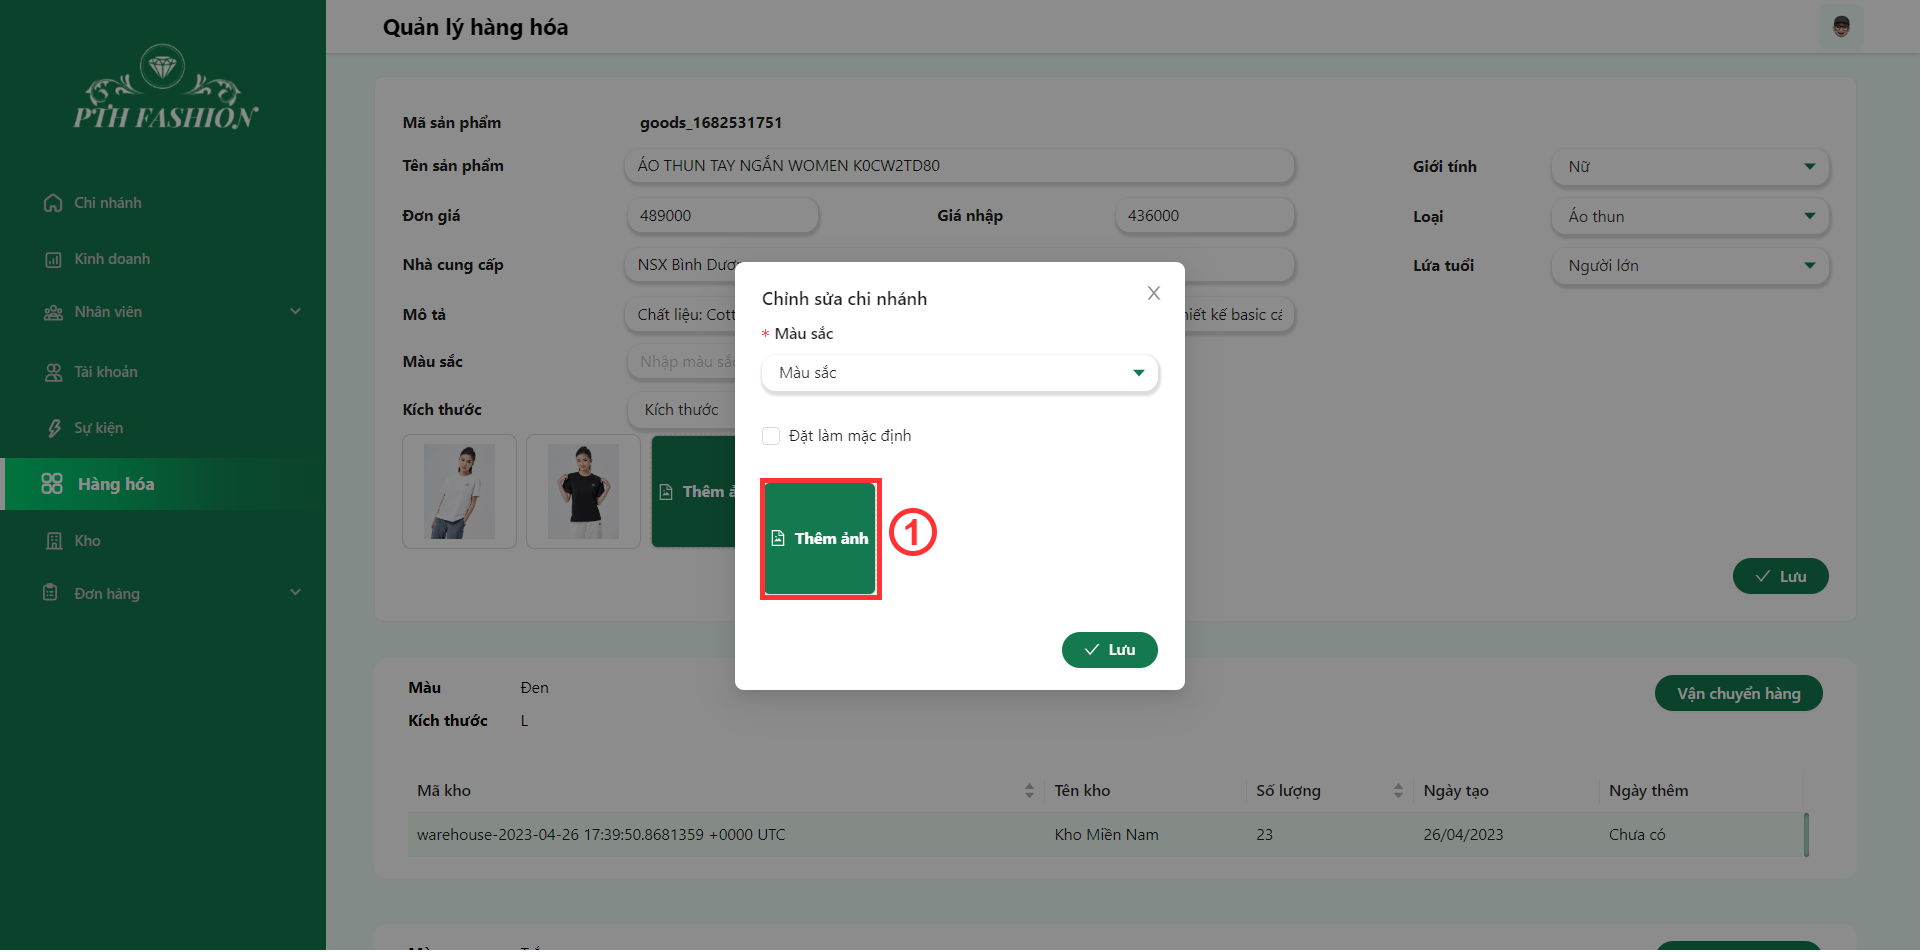
\includegraphics[width=12cm]{img/UI/admin_implement/goodsImage.png}
    \newline
    \caption{Giao diện thêm ảnh cho hàng}
\end{figure}
\textbf{Mô tả:}
\begin{quote}
    \begin{enumerate}
        \item Chọn để tải ảnh lên
    \end{enumerate}
\end{quote}

\subsubsubsection{Vận chuyển hàng}
\begin{figure}[!htp]
    \centering
    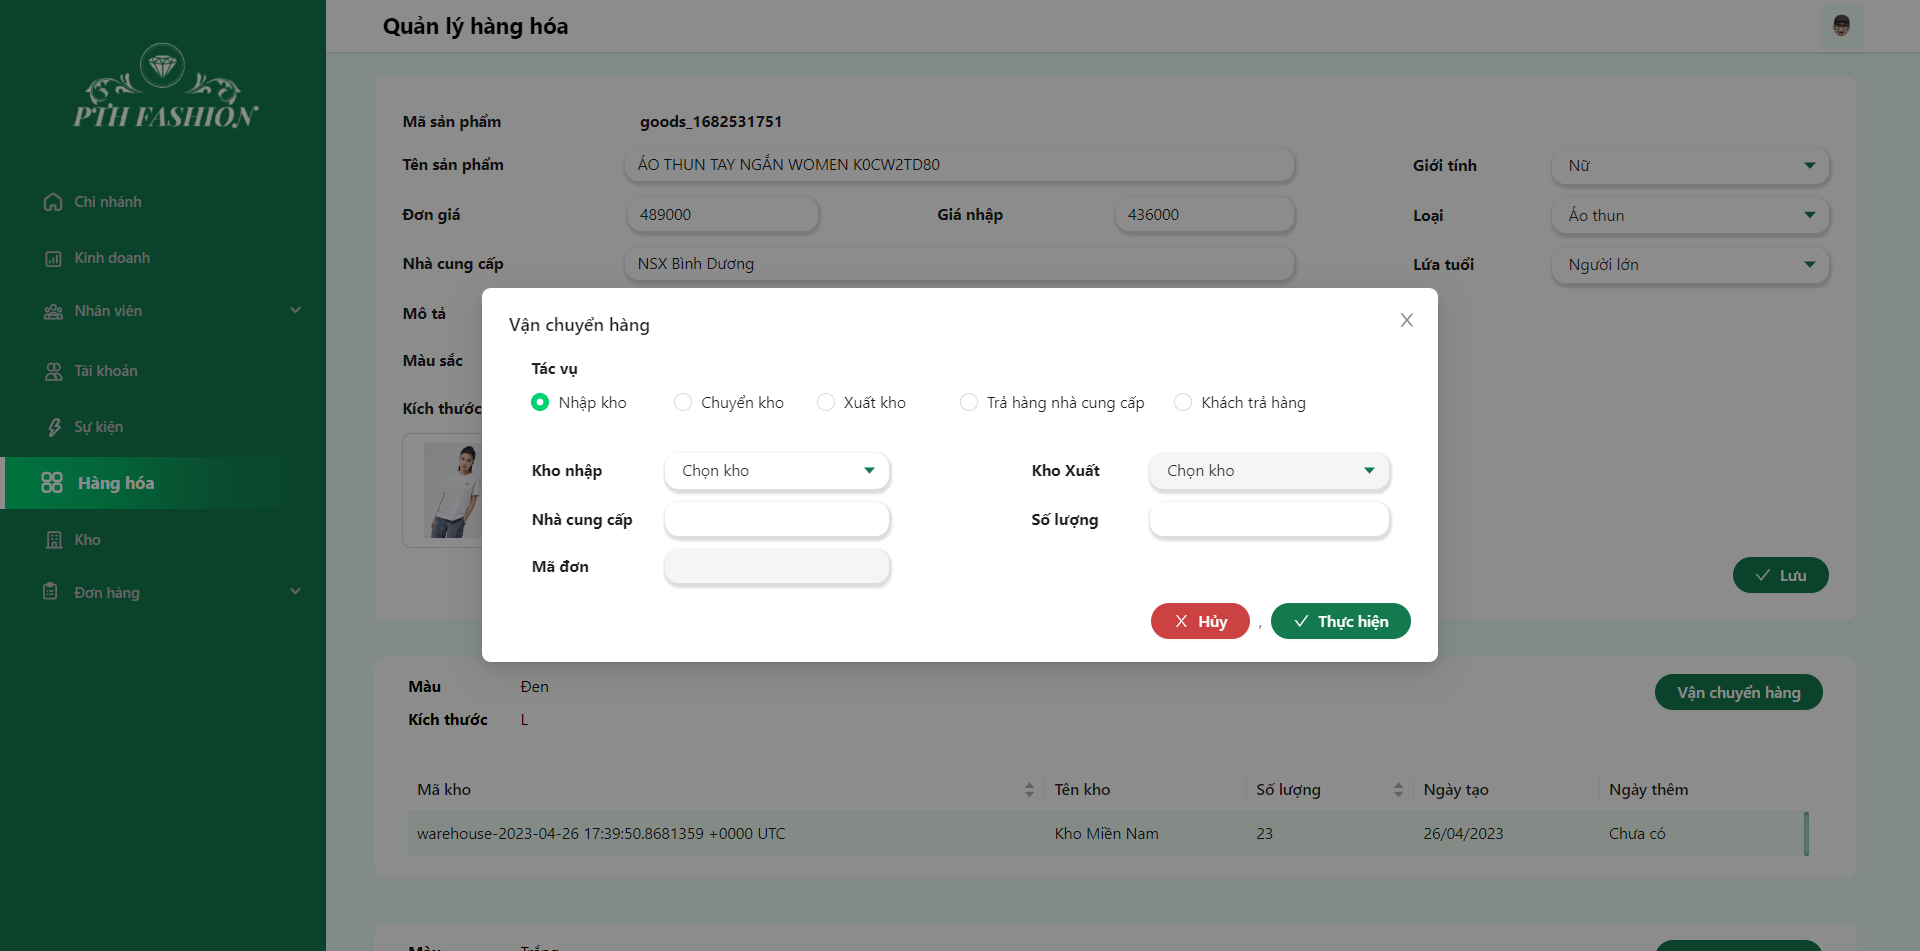
\includegraphics[width=12cm]{img/UI/admin_implement/goodsTransfer.png}
    \newline
    \caption{Giao diện vận chuyển hàng}
\end{figure}
\textbf{Mô tả:}
\begin{quote}
    Người dùng có thể thực hiện nhập kho, chuyển kho, xuất kho, nhận hàng và trả hàng
\end{quote}

\newpage

\subsubsection{Quản lý đơn hàng}
\begin{figure}[!htp]
    \centering
    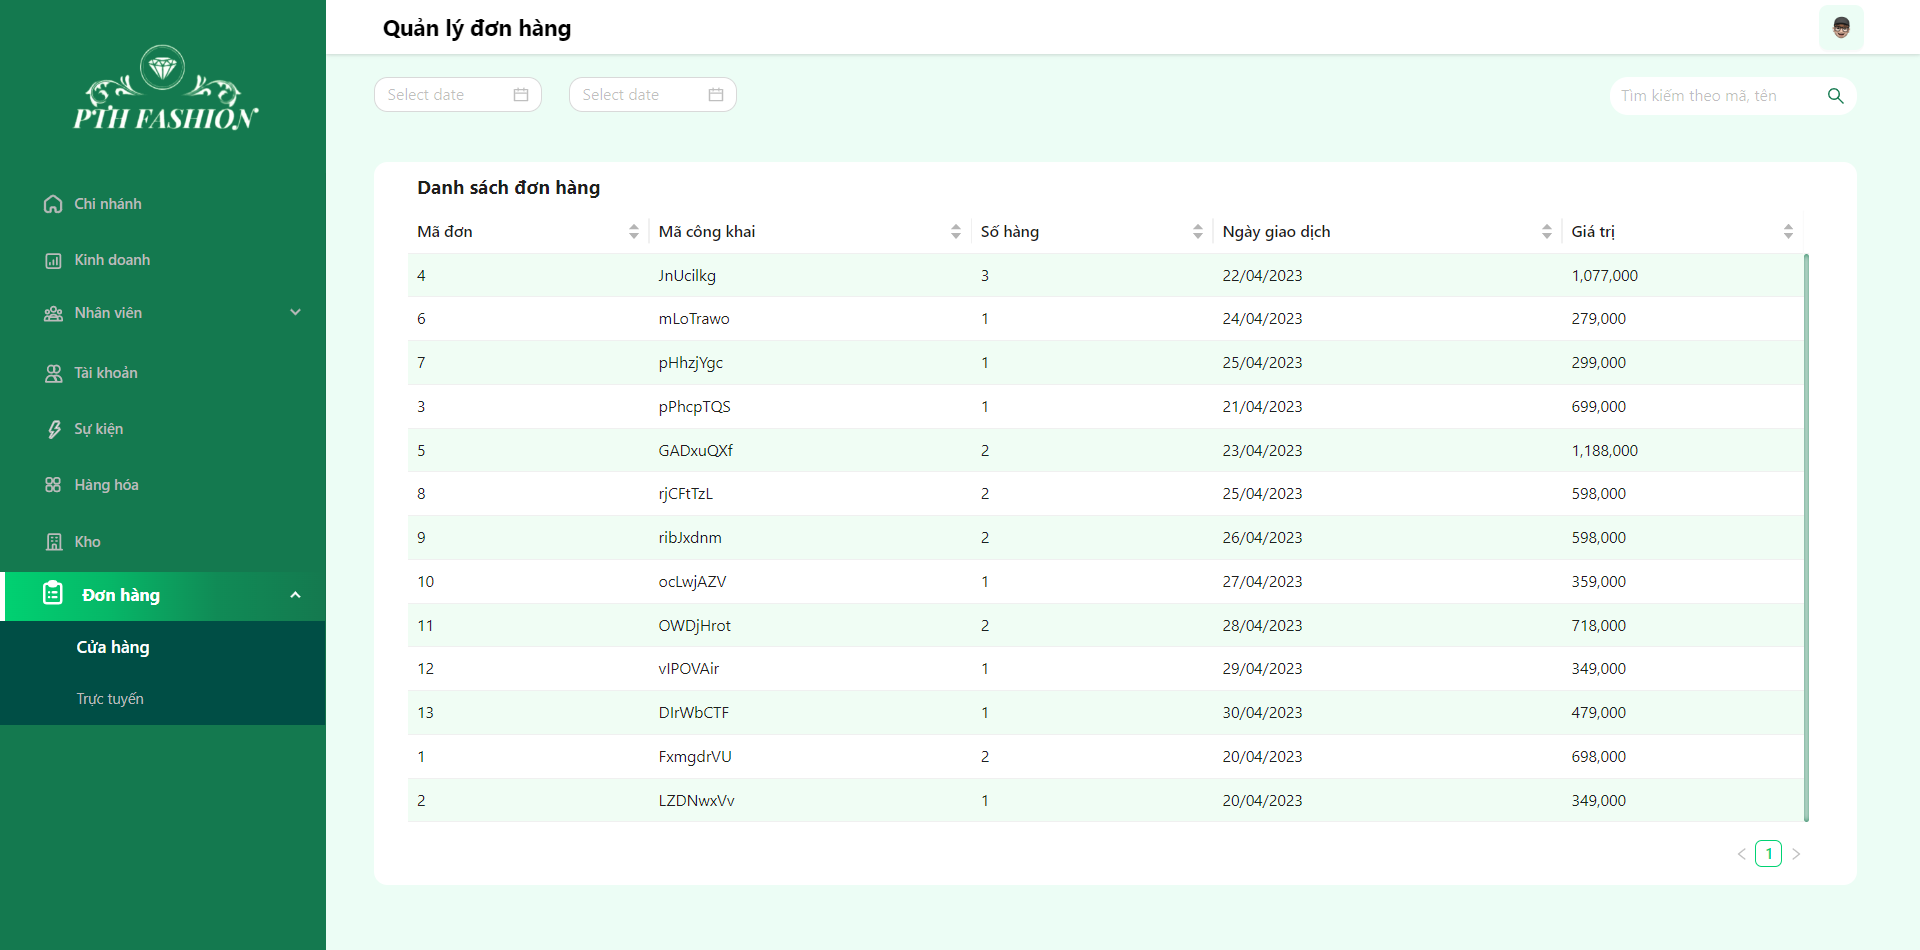
\includegraphics[width=12cm]{img/UI/admin_implement/order.png}
    \newline
    \caption{Giao diện quản lý đơn hàng}
\end{figure}

\subsubsubsection{Chi tiết đơn hàng}
\begin{figure}[!htp]
    \centering
    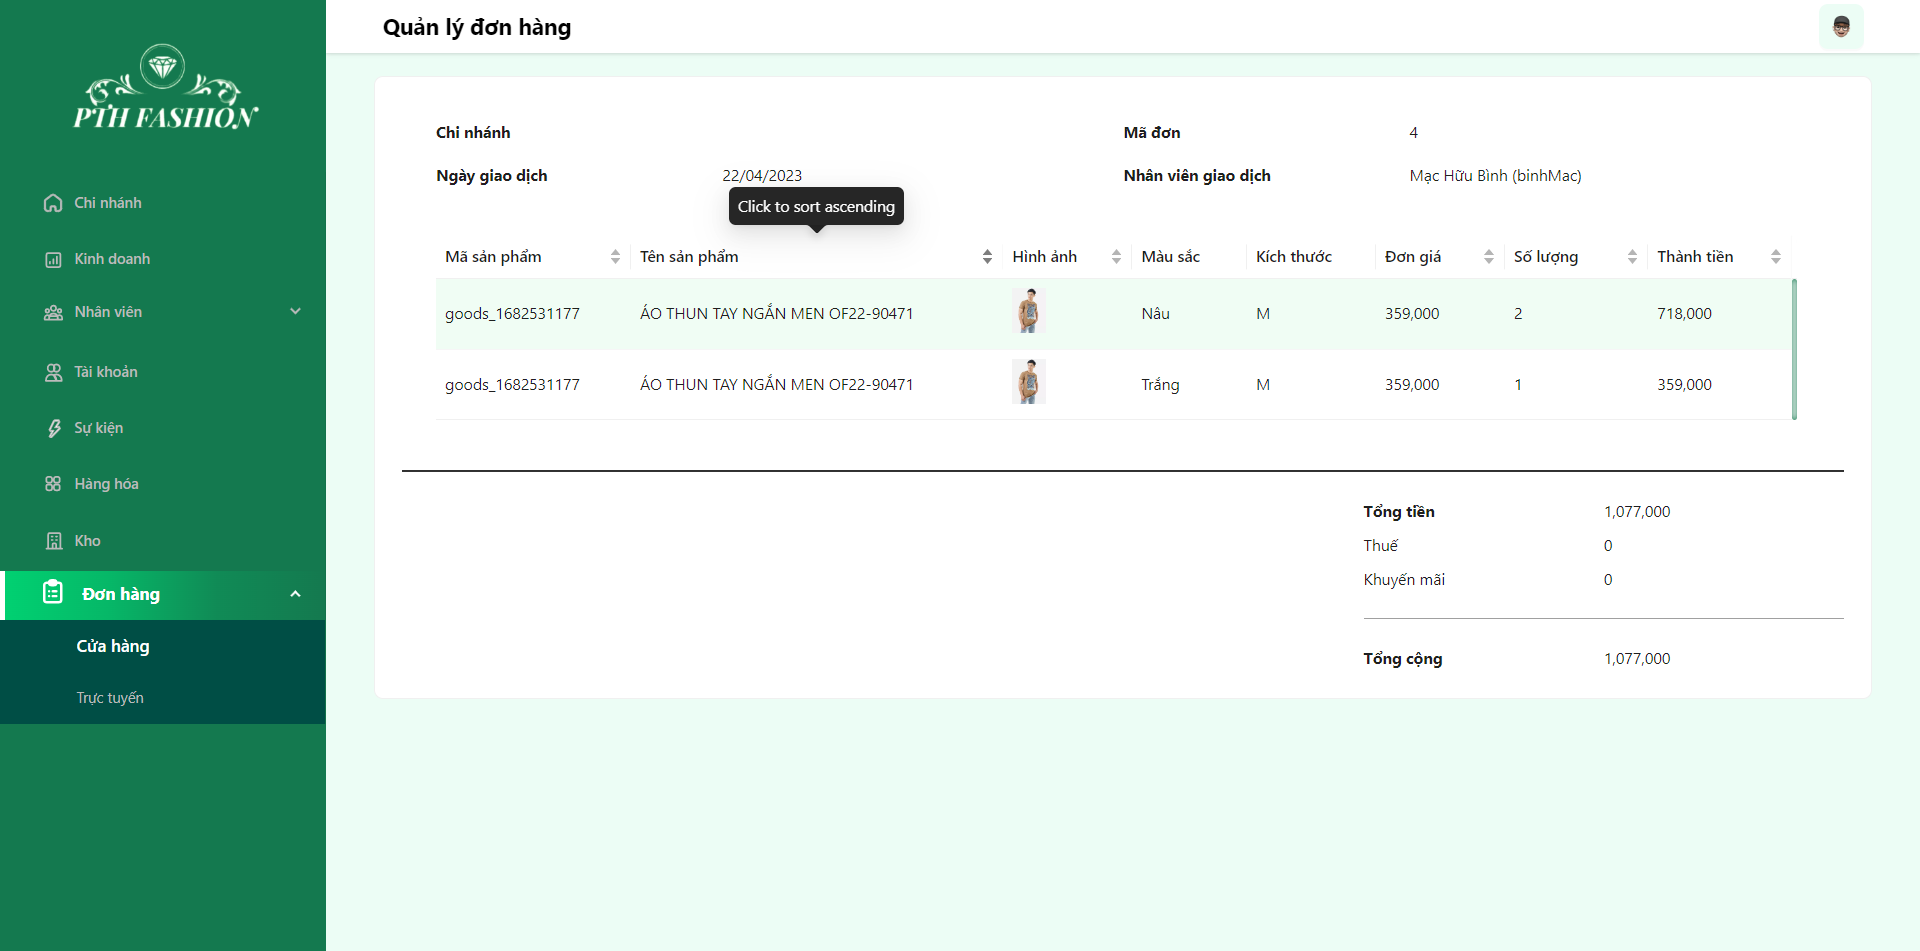
\includegraphics[width=12cm]{img/UI/admin_implement/orderDetail.png}
    \newline
    \caption{Giao diện chi tiết đơn hàng}
\end{figure}

\newpage

% \subsubsection{Quản lý đơn hàng trực tiếp}
% \begin{figure}[!htp]
%     \centering
%     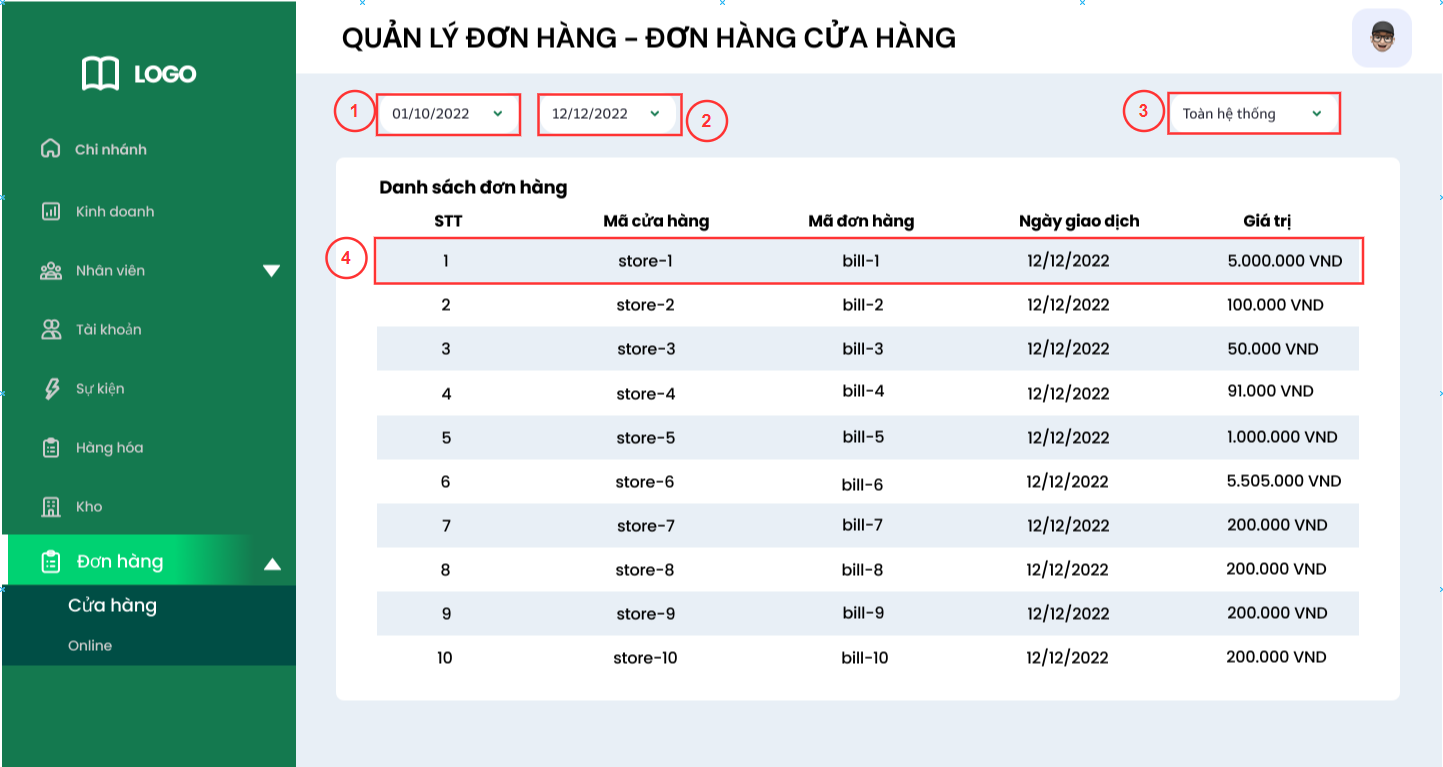
\includegraphics[width=12cm]{img/UI/admin/OfflineOrder.png}
%     \label{42}
%     \newline
%     \caption{Giao diện quản lý đơn hàng cửa hàng}
% \end{figure}
% \textbf{Mô tả:}
% \begin{quote}
%     \begin{enumerate}
%         \item Chọn thời gian bắt đầu
%         \item Chọn thời gian kết thúc
%         \item Nhập để lọc đơn theo mã đơn
%         \item Chọn để xem chi tiết đơn hàng
%     \end{enumerate}
% \end{quote}
% \subsubsubsection{Chi tiết đơn hàng cửa hàng}
% \begin{figure}[!htp]
%     \centering
%     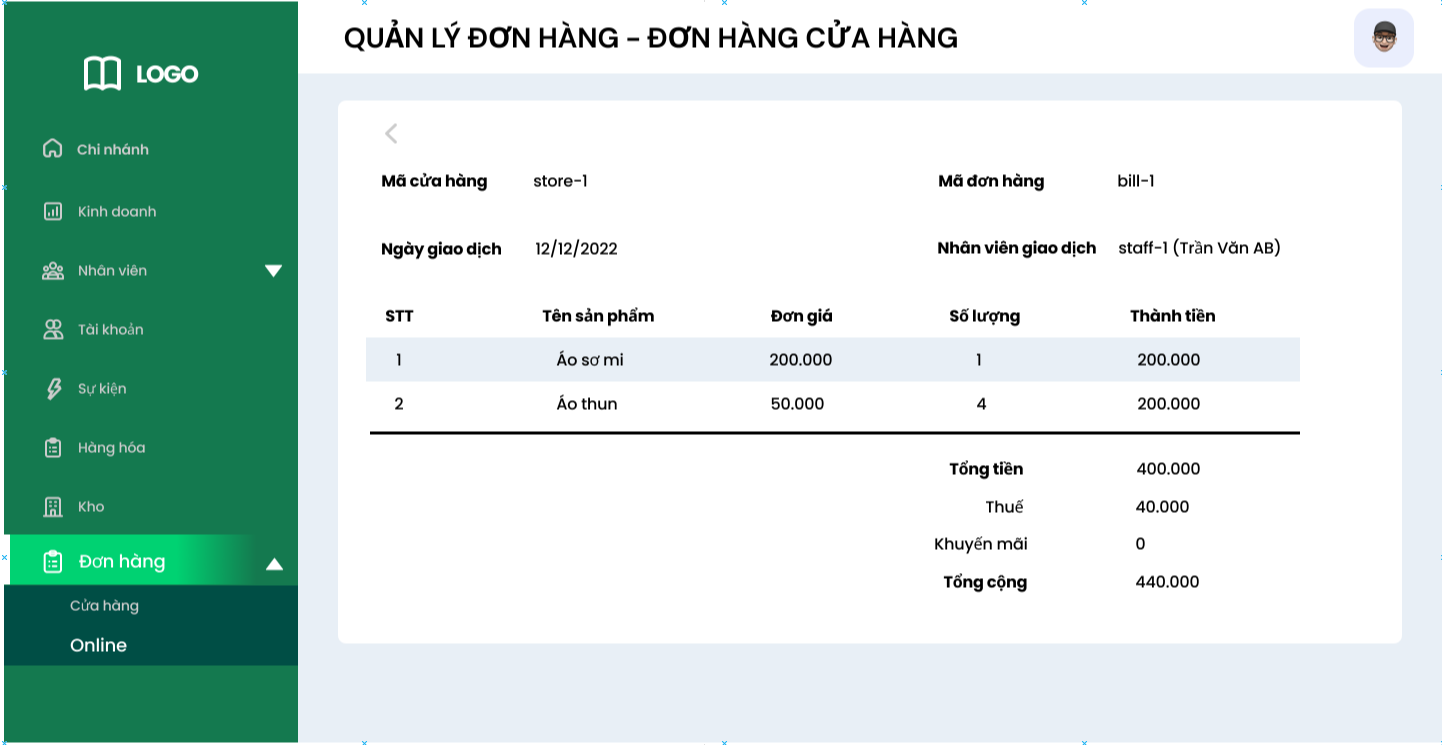
\includegraphics[width=12cm]{img/UI/admin/OfflineOrder_detai;.png}
%     \label{43}
%     \newline
%     \caption{Giao diện chi tiết đơn hàng cửa hàng}
% \end{figure}


\subsubsection{Giao diện khác}
Bên cạnh quản trị viên, quản lý ở cấp cao nhất thì còn các quản lý ở từng mảng và chỉ sử dụng được một vài chức năng của quản trị viên:
\begin{itemize}
    \item Quản lý chi nhánh: Quản lý chi nhánh, quản lý hoạt động kinh doanh, quản lý nhân viên, quản lý đơn hàng cửa hàng
    \item Trưởng chi nhánh: Quản lý hoạt động kinh doanh (riêng chi nhánh), quản lý nhân viên(riêng chi nhánh), quản lý đơn hàng(riêng chi nhánh).
    \item Quản lý hàng hóa: Quản lý hàng hóa
    \item Quản lý kho: Quản lý kho.
\end{itemize}
\subsubsubsection{Quản lý chi nhánh}
\begin{figure}[!htp]
    \centering
    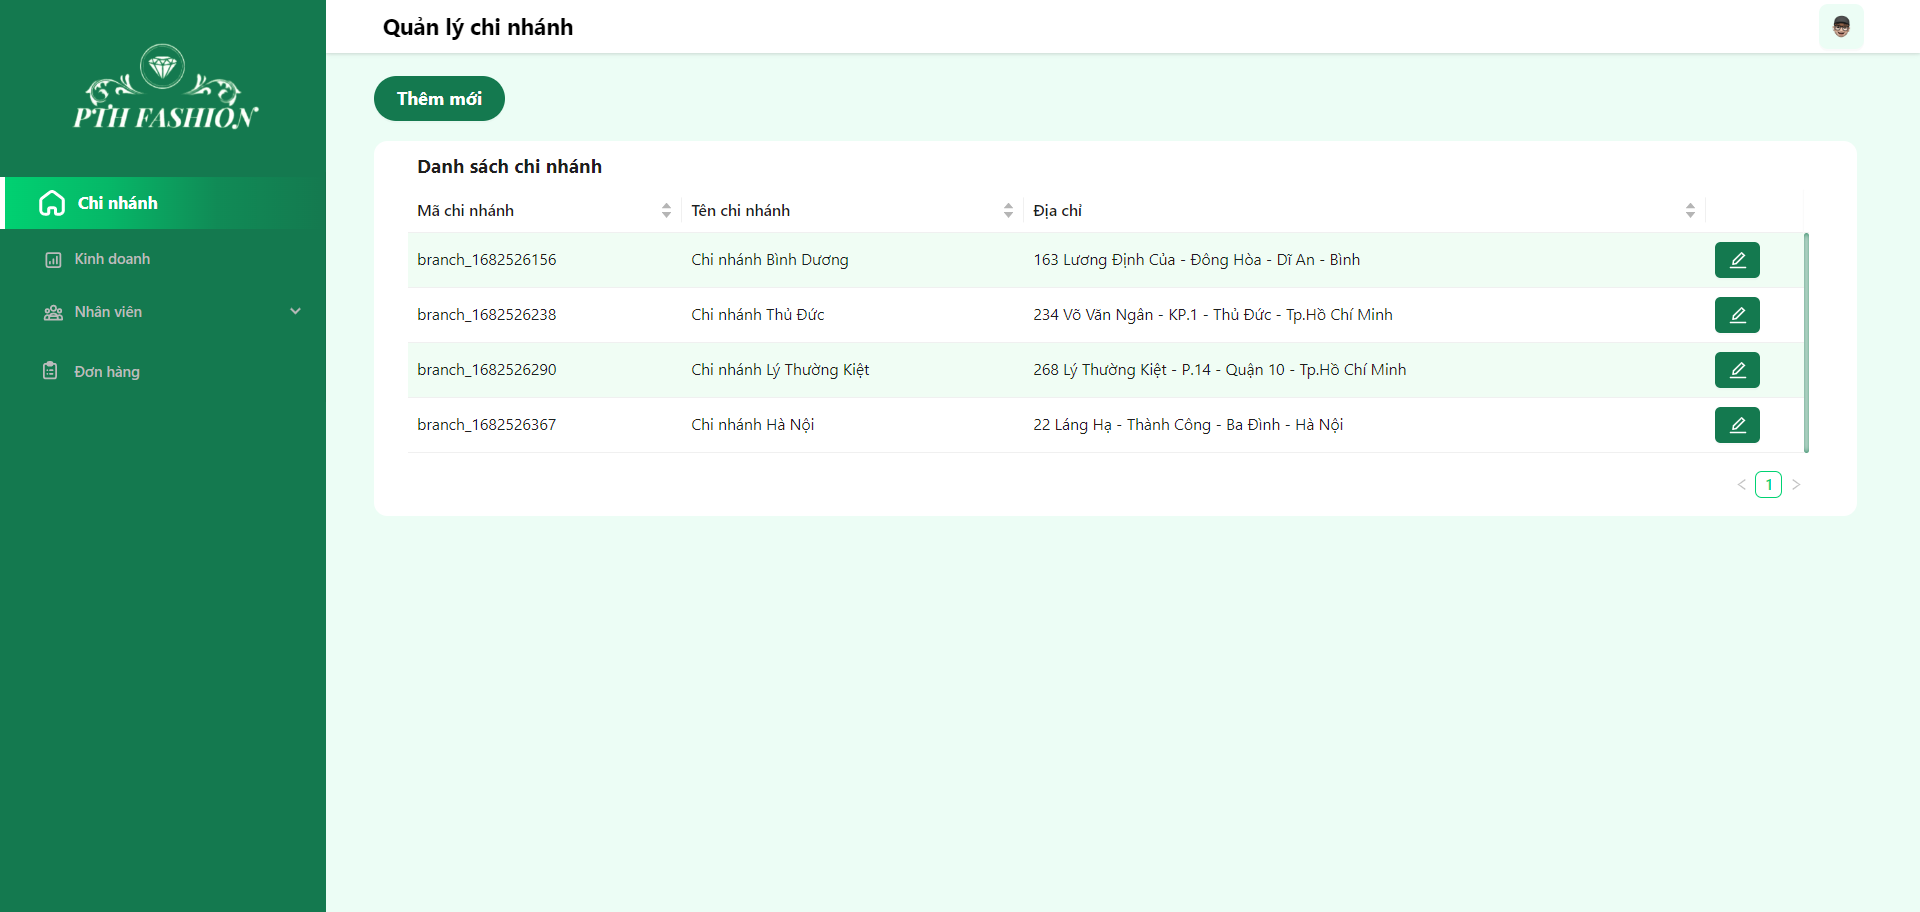
\includegraphics[width=12cm]{img/UI/admin_implement/branchManager.png}
    \newline
    \caption{Giao diện của người quản lý chi nhánh}
\end{figure}

\subsubsubsection{Trưởng chi nhánh}
\begin{figure}[!htp]
    \centering
    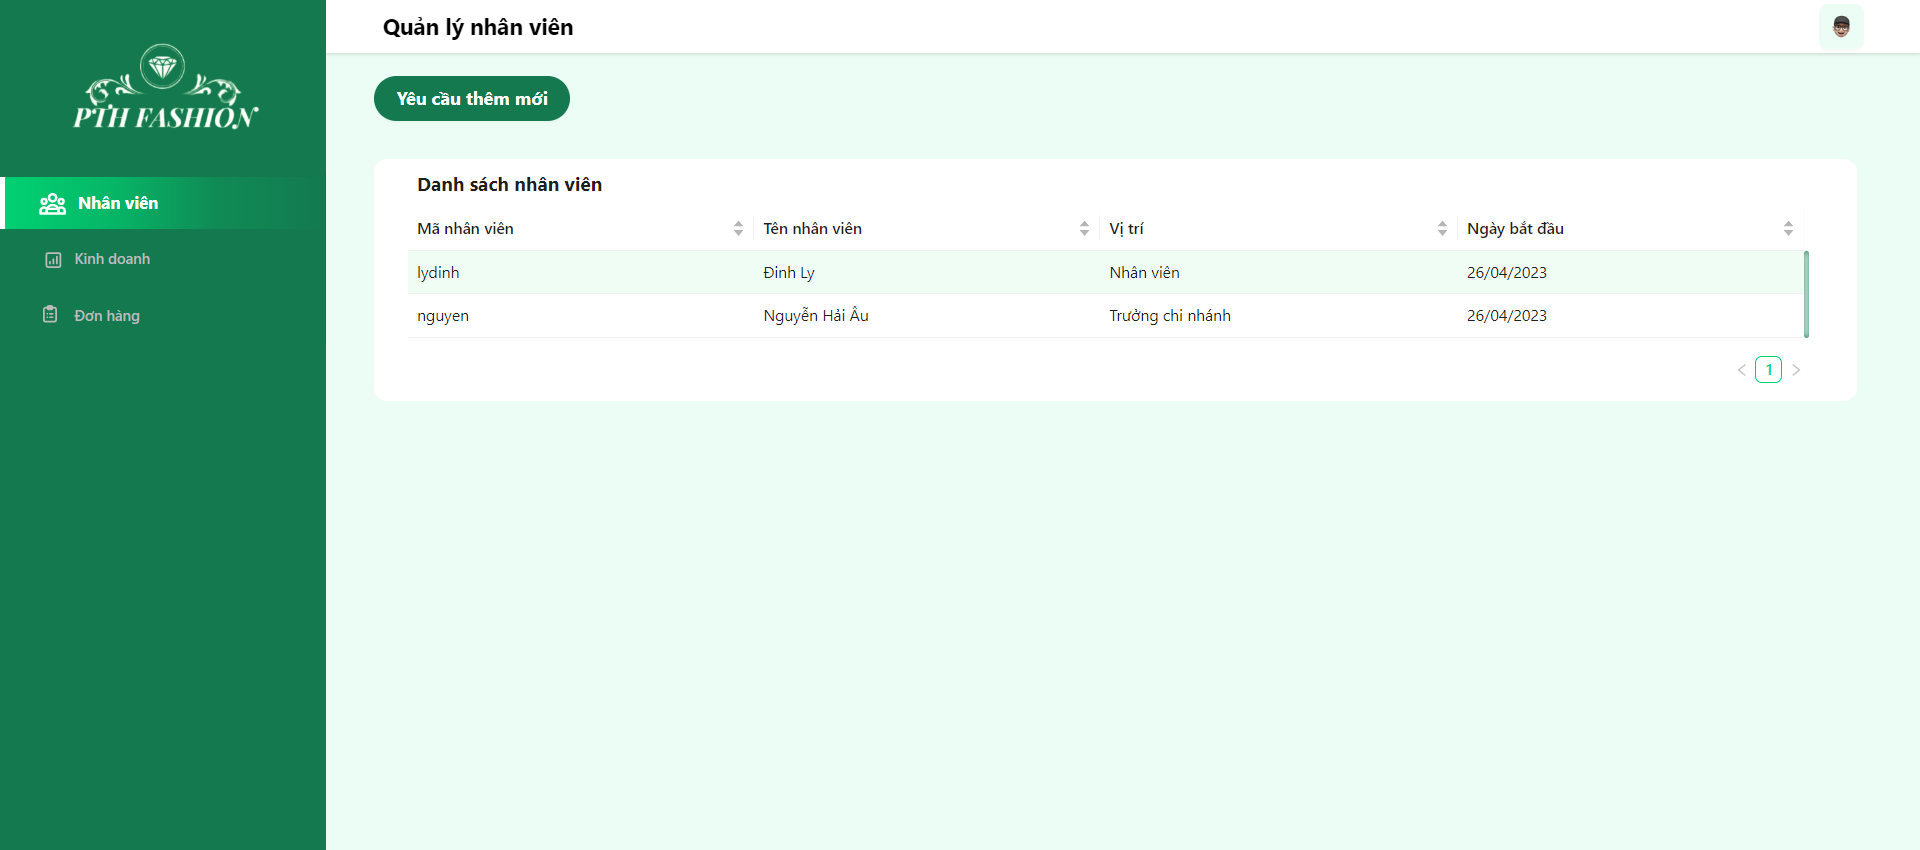
\includegraphics[width=12cm]{img/UI/admin_implement/branchLeader.png}
    \newline
    \caption{Giao diện của người trưởng chi nhánh}
\end{figure}
\newpage


\subsubsubsection{Quản lý hàng hóa}
\begin{figure}[!htp]
    \centering
    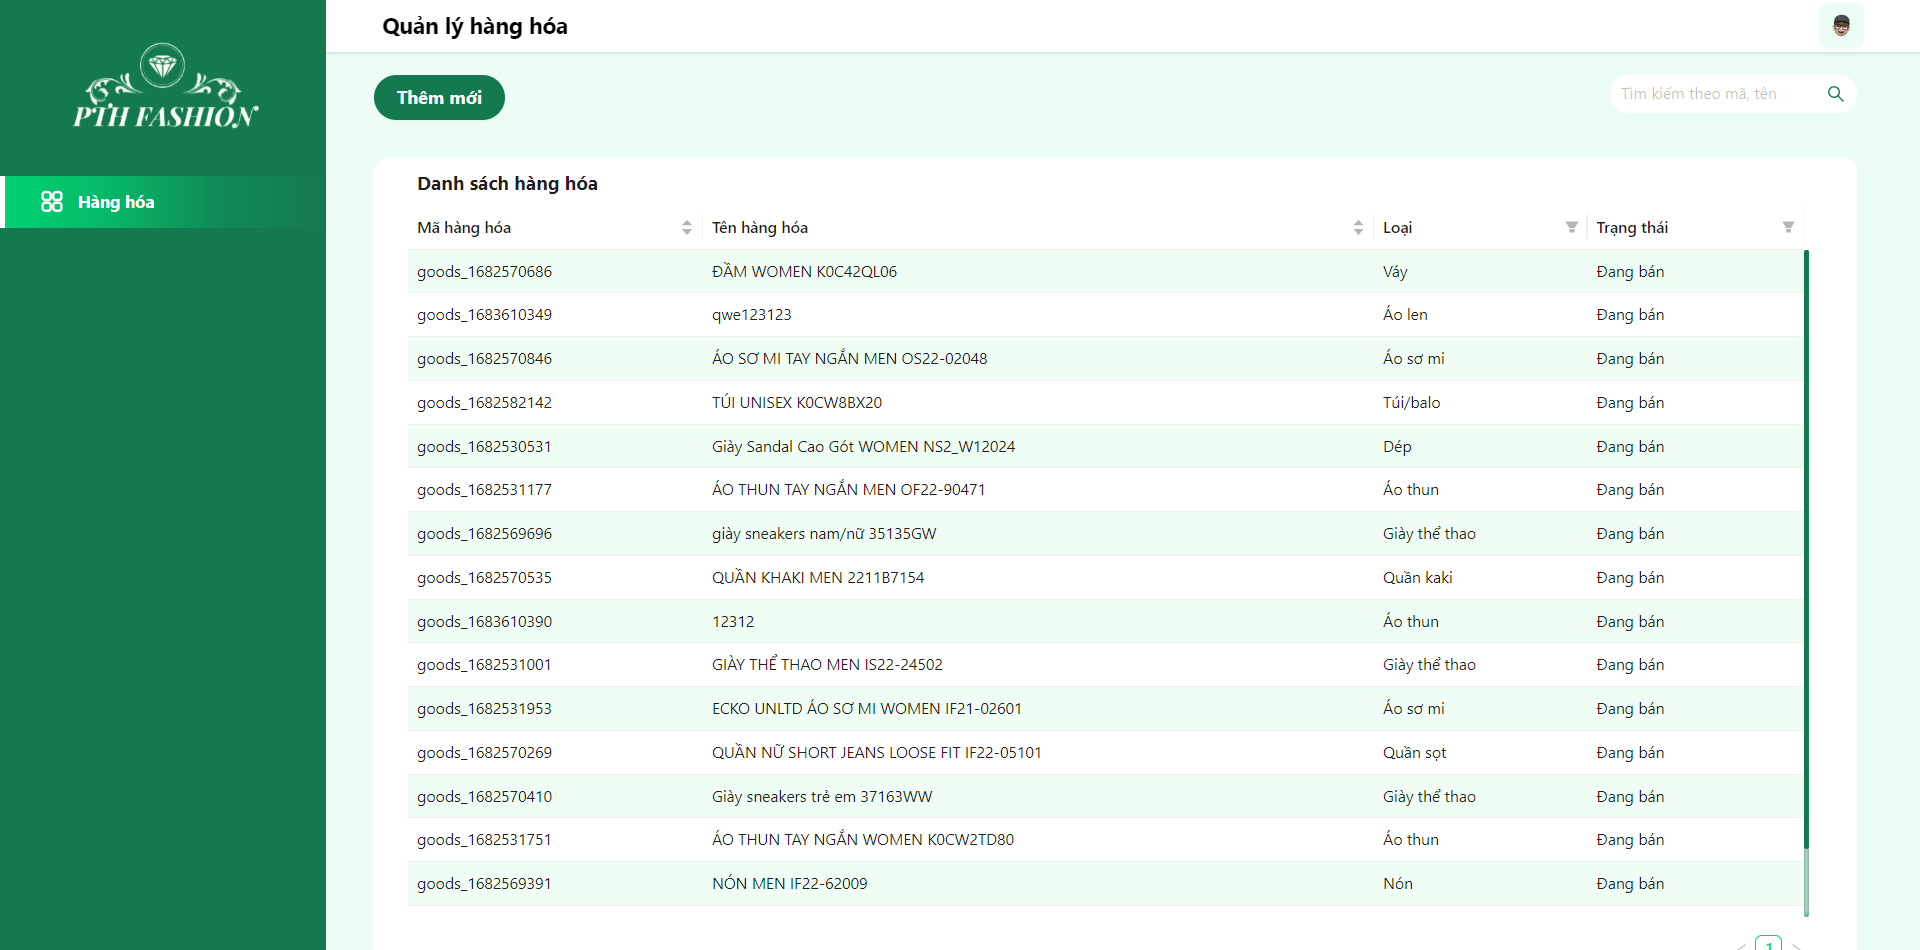
\includegraphics[width=12cm]{img/UI/admin_implement/goodsManager.png}
    \newline
    \caption{Giao diện của người quản lý hàng hóa}
\end{figure}

\subsubsubsection{Quản lý kho}
\begin{figure}[!htp]
    \centering
    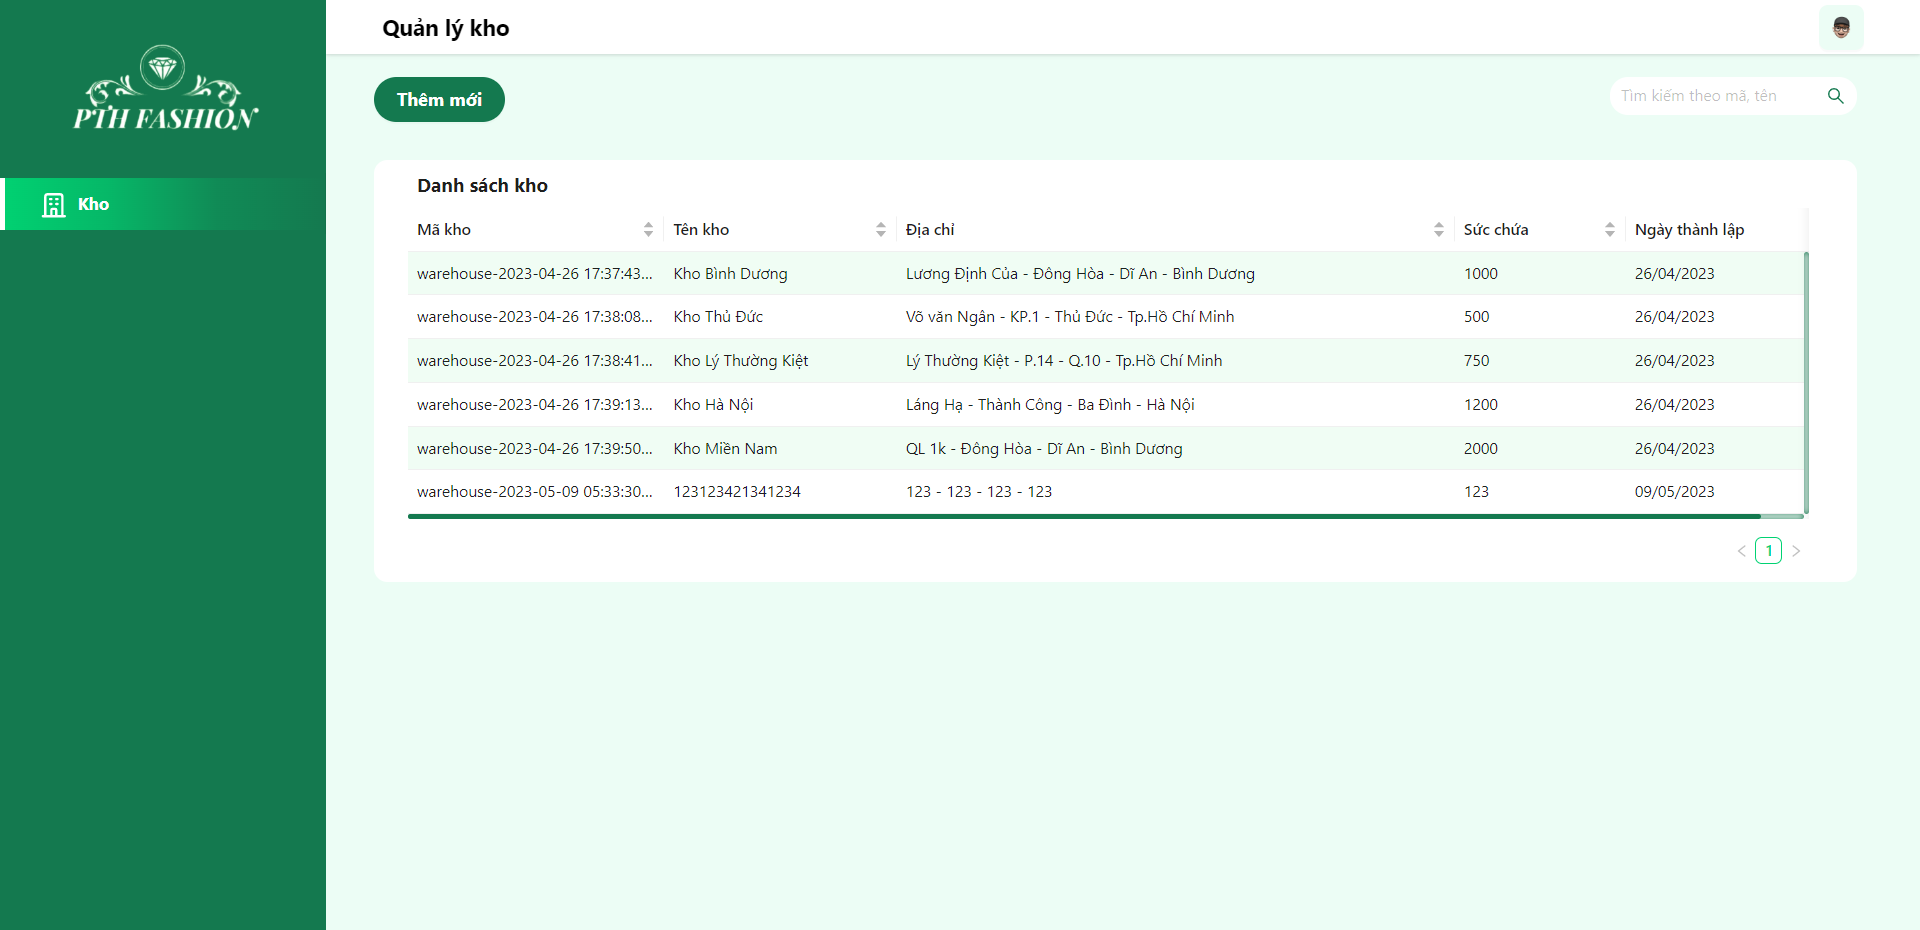
\includegraphics[width=12cm]{img/UI/admin_implement/warehouseManager.png}
    \newline
    \caption{Giao diện của người quản lý kho }
\end{figure}


